% --------------------------------------------------
% 
% This chapter is for PEMA and DARN 
% 
% --------------------------------------------------

\chapter{Software development to establish quality HTS-oriented bioinformatics methods for microbial diversity assessment}
\label{cha:2}


% ----------------------------------------
% 
%      PEMA
% 
% ----------------------------------------
% SECTION 2
\section[PEMA: a flexible Pipeline for Environmental DNA Metabarcoding Analysis of the 16S/18S ribosomal RNA, ITS, and COI marker genes]{
   PEMA: a flexible Pipeline for Environmental DNA Metabarcoding Analysis of the 16S/18S ribosomal RNA, ITS, and COI marker genes~\footnote{
      For author contributions, please refer to the relevant section. Modified version of the published review; extra features have been added and discussed on this thesis.\\
      You may find the Supplementary files of this study through 
      \href{https://academic.oup.com/gigascience/article/9/3/giaa022/5803335\#supplementary-data}{PEMA's publication}
      (\href{https://academic.oup.com/gigascience/article/9/3/giaa022/5803335\#supplementary-data}{https://academic.oup.com/gigascience/article/9/3/giaa022/5803335\#supplementary-data})
      Here a modified version of the published version is presented in terms of relevance, coherence and formatting.
   }
}
\label{publ:pema}

   \textbf{Citation:} \\ 
   Zafeiropoulos, H., Viet, H.Q., Vasileiadou, K., Potirakis, A., Arvanitidis, C., Topalis, P., Pavloudi, C. and Pafilis, E., 2020. PEMA: a flexible Pipeline for Environmental DNA Metabarcoding Analysis of the 16S/18S ribosomal RNA, ITS, and COI marker genes. GigaScience, 9(3), p.giaa022, \\ 
   DOI: \href{https://doi.org/10.1093/gigascience/giaa022}{10.1093/gigascience/giaa022}.


   \subsection{Abstract}
   \textbf{Background:} 
   Environmental DNA and metabarcoding allow the identification of a mixture of species and launch 
   a new era in bio- and eco-assessment. 
   Many steps are required to obtain taxonomically assigned matrices from raw data. For most of these, 
   a plethora of tools are available; each tool's execution parameters need to be tailored to reflect each experiment's idiosyncrasy. 
   Adding to this complexity, the computation capacity of high-performance computing systems is frequently required for such analyses. 
   To address the difficulties, bioinformatic pipelines need to combine state-of-the art technologies and 
   algorithms with an easy to get-set-use framework, allowing researchers to tune each study. 
   Software containerization technologies ease the sharing and running of software packages across operating systems; 
   thus, they strongly facilitate pipeline development and usage. 
   Likewise programming languages specialized for big data pipelines incorporate features like roll-back checkpoints and on-demand partial pipeline execution.

   \textbf{Findings:}
   PEMA is a containerized assembly of key metabarcoding analysis tools that requires low effort in setting up, running, and customizing to researchers' needs. 
   Based on third-party tools, PEMA performs read pre-processing, (molecular) operational taxonomic unit 
   clustering, amplicon sequence variant inference, and taxonomy assignment for 16S and 18S ribosomal RNA, as well as ITS and COI marker gene data. 
   Owing to its simplified parameterization and checkpoint support, PEMA allows users to explore alternative algorithms for specific steps of the pipeline without the need of a complete re-execution. 
   PEMA was evaluated against both mock communities and previously published datasets and achieved results of comparable quality.

   \textbf{Conclusions:}
   A high-performance computing–based approach was used to develop PEMA; however, it can be used in personal computers as well. 
   PEMA's time-efficient performance and good results will allow it to be used for accurate environmental DNA metabarcoding analysis, thus enhancing the applicability of next-generation biodiversity assessment studies.
   
   % PEMA INTRODUCITON
   \subsection{Introduction}

   Environmental DNA (eDNA) metabarcoding inaugurates a new era in bio- and eco-monitoring \citep{pavan2015dna}. 
   eDNA refers to genetic material obtained directly from environmental samples (soil, sediment, water, etc.) without any obvious signs of biological source material \citep{thomsen2015environmental}. 
   Metabarcoding is the combination of DNA taxonomy, based on taxa-specific marker genes (e.g., 16S ribosomal RNA [rRNA] for Bacteria and Archaea, cytochrome oxidase subunit 1 [COI] and 18S rRNA for Metazoa, ITS for Fungi), and high-throughput DNA sequencing technologies; thus, simultaneous identification of a mixture of organisms is attainable \citep{ji2013reliable}. 
   eDNA metabarcoding attempts to turn the page on the way biodiversity is perceived and monitored \citep{ji2013reliable}. 
   This combination is considered to be a potential holistic approach that, once standardized, allows for higher detection capacity and at a lower cost compared to conventional methods of biodiversity assessment. 
   However, from the raw read sequence files to an amplicon study's results, the bioinformatics analysis required can be troublesome for many researchers.

   Well-established pipelines are available to process metabarcoding data for the case of 16S and 18S rRNA marker genes and bacterial communities (e.g., mothur \citep{schloss2009introducing}, QIIME 2 \citep{bolyen2018qiime}, LotuS \citep{hildebrand2014lotus}). 
   However, certain limitations accompany each of these and occasionally they can be far from easy-to-use software. Moreover, there is a great need for similarly straightforward and benchmarked approaches for the analysis of other marker genes. With respect to the COI and ITS marker genes, a number of pipelines have been implemented, e.g., 
   \href{https://github.com/enormandeau/barque}{Barque} 
   \footnote{
      \href{https://github.com/enormandeau/barque}{https://github.com/enormandeau/barque}
   }, 
   ScreenForBio~\citep{axtner2019efficient}, and PIPITS~\citep{gweon2015pipits}. 
   However, there is still need for a fast, flexible, easy-to-install, and easy-to-use pipeline for both COI and ITS marker genes.
   
   The pipelines mentioned above, although entrenched, are still hindered by a series of hurdles. 
   Among the most prominent are technical difficulties in installation and use, strict limitations in setting parameters for the algorithms invoked, and incompetence in partial re-execution of an analysis.
   
   Moreover, given the computational demands of such analyses, access to high - performance computing (HPC) systems might be mandatory, e.g., to process studies with a large number of samples. 
   This is timely given the ongoing investment of national and international efforts (
   e.g., see 
   \href{https://www.esfri.eu/sites/default/files/u4/ESFRI_SCRIPTA_VOL3_INNO_double_page.pdf}{European Strategy Forum on Research Infrastructures} \footnote{
      \href{https://www.esfri.eu/sites/default/files/u4/ESFRI_SCRIPTA_VOL3_INNO_double_page.pdf}{https://www.esfri.eu/sites/default/files/u4/ESFRI\_SCRIPTA\_VOL3\_INNO\_double\_page.pdf}
   }
   ) 
   to serve the broad biological community via commonly accessible infrastructures.
   
   % PEMA CONTRIBUTION
   \subsection{Contribution}

   PEMA (Pipeline for Environmental DNA Metabarcoding Analysis) is an open source pipeline 
   that bundles state-of-the-art bioinformatic tools for all necessary steps of amplicon analysis 
   and aims to address the aforementioned issues. 
   It is designed for paired-end sequencing studies and is implemented in the 
   BDS~\citep{cingolani2015bigdatascript} programming language. 
   BDS's ad hoc task parallelism and task synchronization supports heavyweight computation, 
   which PEMA inherits. 
   In addition, BDS supports "checkpoint" files that can be used for partial re-execution 
   and crash recovery of the pipeline. 
   PEMA builds on this feature to serve tool and parameter exploratory customization 
   for optimal metabarcoding analysis fine tuning.
   Switching effortlessly between (molecular) operational taxonomic unit ([M]OTU) clustering 
   and amplicon sequence variant (ASV) inference algorithms is a pertinent example. 
   Finally, via software containerization technologies such as Docker~\citep{rad2017introduction} 
   and Singularity~\citep{kurtzer2017singularity}, with the latter being HPC-centered, 
   PEMA is distributed in an easy to download and install fashion on a range of systems, 
   from regular computers to cloud or HPC environments.
   
   From the biological perspective, monitoring biodiversity at all its different levels 
   is of great importance. 
   Because there is not a single marker gene to detect all taxa, researchers need to use 
   different genes targeting each great taxonomy group separately~\citep{coissac2012bioinformatic}. 
   To that end, PEMA supports the metabarcoding analysis of both prokaryotic communities, 
   based on the 16S rRNA marker gene, and eukaryotic ones, based on the ITS (for Fungi) 
   and COI and 18S rRNA (for Metazoa) marker genes~\citep{coissac2012bioinformatic}.
   
   As high-throughput sequencing (HTS) data become more and more accurate, ASVs, 
   i.e., marker gene amplified sequence reads that differ in $≥1$ nucleotide from each other, 
   become easier to resolve~\citep{callahan2017exact}. 
   The use of ASVs instead of OTUs has been suggested~\citep{callahan2017exact}; 
   however, the choice of which approach to use should be based on each study's 
   objective(s) \citep{pauvert2019bioinformatics}.
   
   PEMA supports both OTU clustering and ASV inference for all marker genes 
   (see “OTU clustering vs ASV inference” in the “Results and Discussion” section). 
   Two clustering algorithms, VSEARCH~\citep{rognes2016vsearch} and CROP~\citep{hao2011clustering}, 
   are used for the clustering of reads in (M)OTUs—the former for the case of 
   the 16S/18S rRNA marker genes, the latter for the case of COI and ITS. 
   Swarm v2~\citep{mahe2015swarm} allows ASV inference in all cases.
   
   Taxonomic assignment is performed in an alignment-based approach, making use of the 
   CREST LCAClassifier \citep{lanzen2012crest} and the Silva database~\citep{quast_silva_2013} 
   for the case of 16S and 18S rRNA marker genes; 
   the Unite database \citep{nilsson2019unite} is used for the ITS gene. 
   In the 16S marker gene case, phylogeny-based assignment is also supported, based on 
   RAxML-ng \citep{kozlov2019raxml}, 
   EPA-ng \citep{barbera2019epa}, and Silva \citep{quast_silva_2013}. 
   For the COI marker gene, the RDPClassifier \citep{wang2007naive} and the 
   MIDORI database \citep{machida2017metazoan} are used for the taxonomic assignment. 
   In addition, ecological and phylogenetic analysis are facilitated via the \texttt{phyloseq} 
   R package \citep{mcmurdie2013phyloseq}.
   
   All the pipeline- and third-party module–controlling parameters are defined in a 
   plain "parameter-value pair" text file. 
   Its straightforward format eases the analysis fine tuning, complementary to the 
   aforementioned checkpoint mechanism. A tutorial about PEMA and installation guidance 
   can be found on \href{https://github.com/hariszaf/pema}{PEMA's GitHub repository} 
   \footnote{
      \href{https://github.com/hariszaf/pema}{https://github.com/hariszaf/pema}
   }.


   % PEMA METHODS
   \subsection{Methods \& Implementation}

   PEMA's architecture comprises 4 main parts taking place in tandem (Figure~\ref{fig:pema-nutshell}). A detailed description of the tools invoked by PEMA and their licenses is included in Additional File 1: Supplementary Methods.

   \begin{figure}[h]
      \centering
      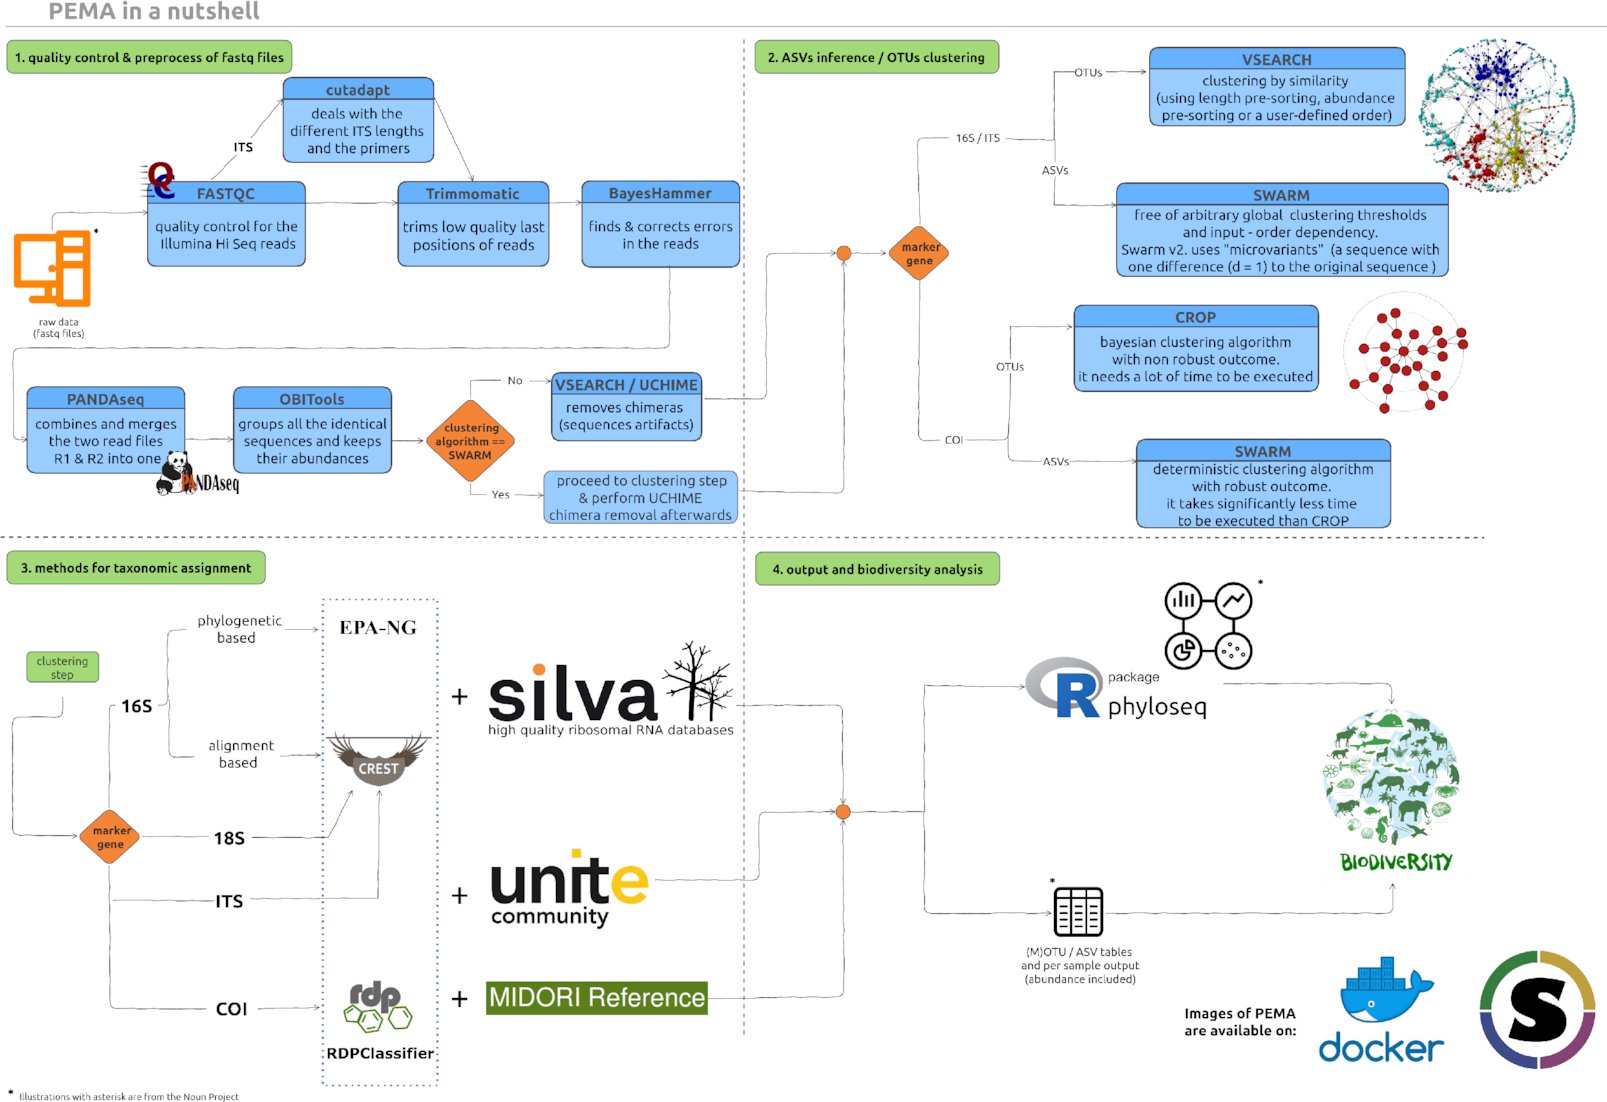
\includegraphics[width=0.95\columnwidth]{figures/pema_workflow.jpeg}
      \caption[PEMA in a nutshell]{PEMA comprises 4 parts. The first step (top left) is the quality control and pre-processing of the Illumina sequencing reads. This step is common for both 16S rRNA and COI marker genes. The second step (top right) is the clustering of reads to (M)OTUs or their inferring to ASVs. The third step (bottom left) is the taxonomy assignment to the generated (M)OTUs/ASVs. In the fourth step (bottom right), the results of the metabarcoding analysis are provided to the user and visualized. *noun project icons by: ProSymbols (US), IconMark (PH), Nithinan Tatah (TH). clustering figure adapted from 
      DOI: \href{https://peerj.com/articles/1420/\#fig-1}{10.7717/peerj.1420/fig-1}}
      \label{fig:pema-nutshell}
   \end{figure}


   \subsubsection*{Part 1: Quality control and pre-processing of raw data}

   First, FastQC \citep{fastqc} is used to obtain an overall read-quality summary; 
   visual inspection of each sample's quality may recommend removing those insufficient quality, 
   as well as samples with a low number of reads, and rerunning the analysis. 
   To correct errors produced by the sequencer, PEMA incorporates a number of tools. 
   Trimmomatic \citep{bolger2014trimmomatic} implements a series of trimming steps, 
   which either remove parts of the sequences corresponding to the adapters or the primers, 
   trim and crop parts of the reads, or even remove a read completely, when it fails to reach 
   the quality-filtering standards set by the user. 
   Cutadapt \citep{martin_cutadapt_2011} is used additionally for the case of ITS to address 
   the variability in length of this marker gene (see Additional File 1: Supplementary Methods). 
   BayesHammer \citep{nikolenko2013bayeshammer}, an algorithm of the 
   SPAdes assembly toolkit \citep{bankevich2012spades}, revises incorrectly called bases. 
   PANDAseq \citep{masella2012pandaseq} assembles the overlapping paired-end reads, 
   and then the \texttt{obiuniq} program of OBITools \citep{boyer2016obitools} groups 
   all the identical sequences in every sample, keeping track of their abundances. 
   The VSEARCH package \citep{rognes2016vsearch} is then invoked for chimera removal; 
   however, if the Swarm v2 algorithm is selected, this step will be performed 
   after the ASV inference (see next section).


   \subsubsection*{Part 2: (M)OTU clustering and ASV inference}

   Quality-controlled and processed sequences are subsequently clustered into (M)OTUs or 
   treated as input for inferring ASVs. 
   For the case of 16S and 18S rRNA marker genes, VSEARCH \citep{rognes2016vsearch} 
   is used for OTU clustering, while ASVs can be identified by the 
   Swarm v2 algorithm \citep{mahe2015swarm}. 
   VSEARCH is an accurate and fast tool that can handle large datasets; 
   at the same time it is a great alternative for USEARCH \citep{edgar2010search} 
   because it is distributed under an open source license.

   For the ITS and COI marker genes, CROP \citep{hao2011clustering}, 
   an unsupervised probabilistic Bayesian clustering algorithm that models 
   the clustering process using birth-death Markov chain Monte Carlo (MCMC), is used. 
   The CROP clustering algorithm is adjusted by a series of parameters that need to be 
   tuned by the user (namely, $b$, $e$, and $z$).
   These parameters depend on specific dataset properties such as the length 
   and the number of reads. 
   PEMA automatically adjusts $b$, $e$, and $z$ by collecting such information 
   and applying the CROP recommended parameter-setting rules \citep{hao2011clustering}. 
   ASV inference is conducted by Swarm v2 \citep{mahe2015swarm} in this case too.

   Because the Swarm v2 algorithm is not affected by chimeras (F. Mahé, personal communication), 
   when Swarm v2 is selected, chimera removal occurs after the clustering 
   (see Additional File 1: Supplementary Methods: Swarm v2). 
   This leads to a computational time gain as chimeras are sought among ASVs, 
   instead of ungrouped reads.

   Last, any singletons, i.e., sequences with only 1 read, occurring after 
   the (M)OTU clustering or the ASV inference may be removed according 
   to the user's parameter settings.


   \subsubsection*{Part 3: Taxonomy assignment}

   Alignment-based taxonomy assignment is supported for all marker gene analyses. 
   In the case of the 16S/18S rRNA and ITS marker genes, the LCAClassifier algorithm of the CREST 
   set of resources and tools [20] is used together with the Silva \citep{quast_silva_2013} 
   and the Unite \citep{nilsson2019unite} database, respectively, to assign taxonomy to the OTUs. 
   Two versions of Silva are included in PEMA: 128 (29 September 2016) and 132 (13 December 2017). 
   Because classifiers need first to be trained for each database they use, 
   for future Silva \citep{quast_silva_2013} versions new PEMA versions will be available.

   For the COI marker gene, PEMA uses the RDPClassifier \citep{wang2007naive} 
   and the MIDORI reference database \citep{machida2017metazoan} to assign taxonomy of the MOTUs. 
   The MIDORI database contains quality-controlled metazoan mitochondrial gene sequences 
   from GenBank \citep{benson2018genbank}.

   Intended primarily for studies from less explored environments, phylogeny - based assignment 
   is available for 16S rRNA marker gene data. 
   PEMA maps OTUs to a custom reference tree of 1,000 Silva-derived consensus sequences 
   (created using RAxML-ng \citep{kozlov2019raxml} and gappa [phat algorithm] \citep{czech2019methods}, 
   Figure~\ref{fig:pema-phylogeny-assignment}A). 
   PaPaRa \citep{berger2012papara} and EPA-ng \citep{barbera2019epa} combine the OTU clustering 
   output and the reference tree to produce a phylogeny-aware alignment and map the 16S rRNA OTUs 
   to the custom reference tree. 
   Beyond the context of PEMA, users may visualize the output with tree viewers 
   such as iTOL \citep{letunic2021interactive} (Figure~\ref{fig:pema-phylogeny-assignment}B).

   \begin{figure}[h]
      \centering
      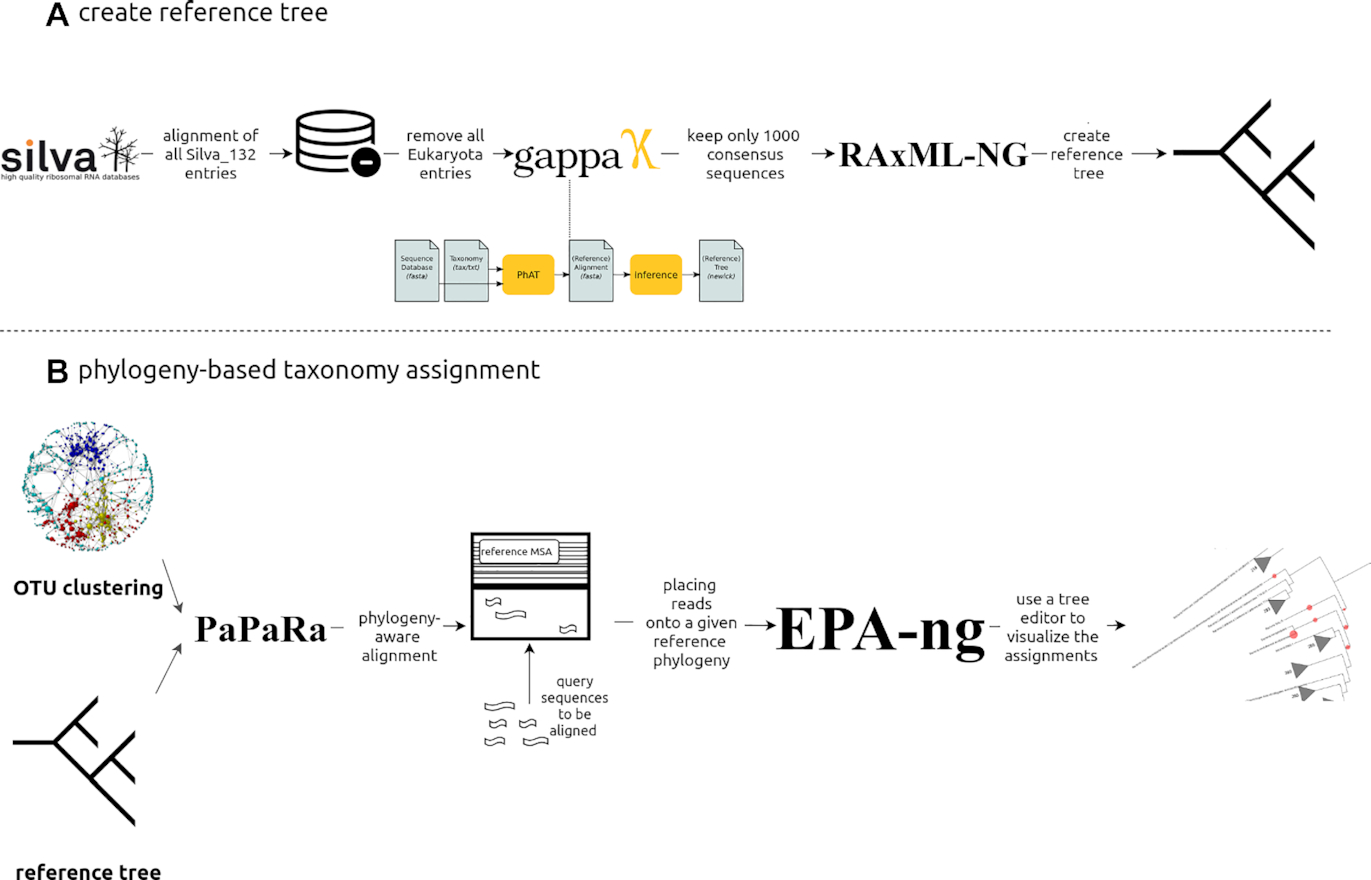
\includegraphics[width=115mm]{figures/pema_phylogenetic_tree.jpeg}
      \caption[Phylogeny - based taxonomy assignment in PEMA]{
         Phylogeny - based taxonomy assignment. 
         A: Building a reference tree for the phylogeny-based taxonomy assignment to 16S rRNA marker gene OTUs: from the latest edition of Silva SSU, all entries referring to Bacteria and Archaea were used and using the “art” algorithm, 10,000 consensus taxa were kept. 
         B: Using PaPaRa and the OTUs that come up from every analysis, an MSA was made and EPA - ng took over the phylogeny - based taxonomy assignment. *noun project icons by: Rockicon and A Beale.
      }
      \label{fig:pema-phylogeny-assignment}
   \end{figure}

   \subsubsection*{Part 4: Ecological downstream analysis of the taxonomically assigned (M)OTU/ASV tables}

   PEMA's major output is either an (M)OTU or an ASV table with the assigned taxonomies 
   and the abundances of each taxon in every sample. 
   For each sample of the analysis, a subfolder containing statistics about the quality of 
   its reads, as well as the taxonomies and their abundances, is also returned.

   Via the \texttt{phyloseq} R package \citep{mcmurdie2013phyloseq}, downstream ecological analysis of the taxonomically assigned OTUs or ASVs is supported. 
   This includes $\alpha-$ and $\beta-$diversity analysis, taxonomic composition, statistical comparisons, and calculation of correlations between samples.

   When selected, in addition to the phyloseq \citep{mcmurdie2013phyloseq} output, a multiple sequence alignment (MSA) and a phylogenetic tree of the OTU/ASVs retrieved can be returned; 
   for the MSA, the MAFFT \citep{katoh2002mafft, nakamura2018parallelization} aligner is invoked while the latter is built by RAxML-ng \citep{kozlov2019raxml}.


   \subsubsection*{PEMA container-based installation}

   An easy way of installing PEMA is via its containers. 
   A Dockerized PEMA version is \href{https://hub.docker.com/r/hariszaf/pema}{available} 
   \footnote{
      \href{https://hub.docker.com/r/hariszaf/pema}{https://hub.docker.com/r/hariszaf/pema}
   }. 
   Singularity users can \textit{pull} the PEMA image from as described in \href{https://github.com/hariszaf/pema}{PEMA GitHub repository}
   \footnote{
      \href{https://github.com/hariszaf/pema}{https://github.com/hariszaf/pema}
   }. 
   Between the 2 containers, the Singularity-based one is recommended for HPC environments owing to Singularity's improved security and file accessing properties, 
   see \href{https://dev.to/grokcode/singularity--a-docker-for-hpc-environments-i6p}{here}
   \footnote{
      \href{https://dev.to/grokcode/singularity--a-docker-for-hpc-environments-i6p}{https://dev.to/grokcode/singularity--a-docker-for-hpc-environments-i6p}
   }. 
   PEMA can also be found in the bio.tools (id: PEMA) and SciCruch (PEMA, \href{https://scicrunch.org/resolver/RRID:SCR_017676}{RRID:SCR\_017676}) databases. 
   For detailed documentation, 
   see \href{https://hariszaf.github.io/pema_documentation/}{here}
   \footnote{
      \href{https://hariszaf.github.io/pema_documentation/}{https://hariszaf.github.io/pema\_documentation/}
   }.

      
   \subsubsection*{PEMA output}

      All PEMA - related files (i.e., intermediate files, final output, checkpoint files, and per - analysis parameters) are grouped in distinct (self - explanatory) subfolders per major PEMA pipeline step. 
      In the last subfolder, i.e., subfolder 8, the results are further split into folders per sample. 
      This eases further analysis both within the PEMA framework (e.g., partial re-execution for parameter exploration) and beyond. 
      An extra subfolder is created when an ecological analysis via the \texttt{phyloseq} package has been selected.

      
   % PEMA RESULTS
   \subsection{Results \& Validation}

   \subsubsection*{Evaluation}

      To evaluate PEMA, 2 approaches were followed. 
      First, PEMA was benchmarked against mock community datasets. 
      Second, PEMA was used to analyse previously published datasets. 
      PEMA's output was then compared with the original study outcome, as well as with the output of QIIME2, LotuS, Mothur, and Barque (where applicable).

      Four mock communities, 1 for each marker gene, were used. With respect to the 16S rRNA marker gene, a mock community of Gohl et al. \citep{gohl2016systematic} with 20 different bacterial species was studied. 
      Correspondingly, in the case of the 18S rRNA marker gene, a mock community of Bradley et al. \citep{bradley2016} with 12 algal species was used; 
      for the ITS, one of Bakker \citep{bakker2018fungal} including 19 different fungal taxa; 
      and for the case of the COI marker gene, a mock community of Bista et al. \citep{bista2018performance} containing 14 metazoan species. 
      More information on the mock communities, their original studies, and the results of PEMA for various combinations of parameters can be found in Additional File 2: Mock Communities.

      Complementary to the mock community evaluation, 2 publicly available datasets from published studies were investigated through PEMA. 
      For the 16S rRNA marker gene, the dataset reported by Pavloudi et al. \citep{pavloudi2017sediment} was used; 
      the original study aimed at investigating the sediment prokaryotic diversity along a transect river–lagoon–open sea. 
      For the COI case, the dataset of Bista et al. \citep{bista2017annual} was used; 
      this study investigated whether eDNA can be used for the accurate detection of chironomids (a taxonomic group of macroinvertebrates) in a freshwater habitat.

      In both approaches, the respective \texttt{.fastq} files were downloaded from the European Nucleotide Archive (ENA) of the European Bioinformatics Institute ENA-(EBI) using \textit{ENA File Downloader version 1.2} \citep{harrison2019european} and PEMA was run on the in-house HPC cluster.

      All analyses were conducted on identical Dell M630 nodes (128 GB RAM, 20 physical Intel Xeon 2.60 GHz cores).


   \subsubsection*{Mock community evaluation}

      PEMA was tested against mock communities. 
      An evaluation of its accuracy must capture 
      (i) how many of PEMA's predictions are true (i.e., the percent of correctly assigned taxa among all predicted taxa) and 
      (ii) how many of the taxa existing in the mock community were recovered successfully by PEMA. 
      The precision statistical metric was used to assess the former, and recall, the latter. 
      In addition, the $F1$-score was used as a combined metric of both precision and recall. 
      Precision is calculated as the ratio of true-positive results (TP) over the total number of true- ($TP$) and false-positive results ($FP$) predicted by a model, as follows: $precision = TP/(TP + FP)$; 
      recall is the ratio of TP over the total number of TP and false-negative results (FN): $recall = TP/(TP + FN)$. 
      The $F1$-score is the precision and recall harmonic mean and is calculated by means of the following formula: 
      $F1 = 2 × (precision × recall)/(precision + recall)$ \citep{sammut2011encyclopedia}.

      Adequate accuracy was achieved when PEMA was used to recover the marker gene – specific mock communities at the genus level.
      Precision and recall scores of ∼80\% or more were observed, with 2 exceptions in precision but also 3 very high scores in recall. 
      Overall the F1-scores ranged from 74\% to 86\%. 
      A detailed description of the benchmark methodology and statistics analysis is given in Additional File 2: Mock Communities.

      Detailed presentation of per-marker-gene–specific mock community recovery via PEMA is provided in the following sections. 
      Several different sets of parameters were chosen for each marker gene. 
      Each marker gene has special features (e.g., length variability, sequence variability), and each Illumina run has its own intrinsic biases (e.g., primers used, PCR protocol); 
      thus, parameter tuning plays a crucial part in metabarcoding analyses.

      In an attempt to thoroughly analyse the sequence data from the mock communities, various sets of parameters were tested on the basis of the experimental details of the published studies but also in an exploratory way. 
      Many different parameter settings were tested, especially for the steps of quality trimming of the reads and the OTU clustering/ASV inference. 
      The differences in their output indicate how sensitive this method is, as well as the great need of a mock community in every metabarcoding study—both as a control but also as a \textit{tuning system} for the parameter setting of the pipeline used.

   \subsubsection*{16S rRNA}

      When PEMA was performed with the Swarm v2 algorithm ($d$ = 3, strictness = 0.6) without removal of singletons, 18 of the 20 taxa were identified to the genus level and 3 of these even to the species level. 
      There were 2 species that were not found in any of the PEMA runs. 
      According to Gohl et al. \citep{gohl2016systematic}, there was a discrepancy in the identification of those 2 species that was dependent on the amplification protocol used. 
      It is worth mentioning that as d increases, taxa cannot be identified to species level at all; 
      however, $FP$ assignments decrease. 
      Thus, when $d$ = 30 and strictness = 0.6 for the KAPA samples, Enterococcus was not identified at all; 
      however, PEMA finds its greatest $F1$ value (at the genus level, see Table~\ref{table:pema-precision}) as the FP assignments returned are minimized. 
      When PEMA was run using the VSEARCH clustering algorithm, high precision values were returned in all cases ($>$0.79). 
      However, the recall values were decreased when using Swarm v2 (0.65–0.68).

      % PEMA MARKER-GENE-SPECIFIC RECOVERY
      \begin{table*}
         \begin{center}
            \begin{tabular}{@{}cccc@{}}
               \toprule
               \multicolumn{1}{c}{\textbf{Marker gene}} & \multicolumn{1}{c}{\textbf{Precision}} & \multicolumn{1}{c}{\textbf{Recall}} & \multicolumn{1}{c}{\textbf{F1}} \\ \midrule
               16S rRNA & 0.81 & 0.85 & 0.83 \\
               18S rRNA & 0.75 & 0.90 & 0.82 \\
               ITS & 0.79 & 0.94 & 0.86 \\
               COI & 0.62 & 0.93 & 0.74
               \end{tabular}
               \caption[Summary benchmark of PEMA marker - gene - specific mock community recovery]{Summary benchmark of PEMA marker - gene – specific mock community recovery (precision)}
               \label{table:pema-precision}
         \end{center}
      \end{table*}




   \subsubsection*{18S rRNA}

      When PEMA was performed using the Swarm v2 algorithm ($d$ = 1, strictness = 0.5), 3 of 12 community members were identified to species level (\textit{Isochrysis galbana}, \textit{Nannochloropsis oculata}, and \textit{Thalassiosira pseudonana}), 6 to genus, and the remaining 3 to class; 
      the latter were all the green algae species (Chlorophyta) of the mock community. 
      However, a better $F1$-score ($0.82$) was achieved when the class of Chlorophyceae was not found at all ($d$ = 1, strictness = 0.3) because the FPs were decreased to only $1$. 
      When the VSEARCH algorithm was used, \textit{I. galbana} was identified only to the genus level, the \textit{Nannochloropsis} to the order level (Eustigmatales), and the \textit{Poterioochromonas} genus to its class (Chrysophyceae).


   \subsubsection*{ITS}

      When PEMA was performed using the Swarm v2 algorithm ($d$ = 20) and targeting the ITS2 region, ASVs from 5 of the 19 species of the mock community were assigned to species level, $10$ to genus, $2$ to family, and $2$ to class level. 
      Contrary to the study by Bakker \citep{bakker2018fungal}, PEMA identified the genus Chytriomyces in all $3$ samples, as well as the Ustilaginaceae family. 
      Only $1$ FP assignment was recorded. 
      When the CROP algorithm was used, PEMA's output was less accurate; 
      the \textit{Fusarium} species contained in the mock community were not identified further than their family (Nectriaceae). 
      As mentioned by Bakker \citep{bakker2018fungal}, many reads deriving from the \textit{Fusarium spp.} were not assigned to species level because of the quality-trimming step. 
      In addition, a manually assembled reference database for the taxonomy assignment was used in the initial study, containing only sequences of the mock community species, which biased this step, making the results not directly comparable to our case.


   \subsubsection*{COI}

      When PEMA was performed on the Bista et al. dataset \citep{bista2018performance} and using Swarm v2 ($d$ = 10), it identified $12$ of the $14$ species included in the mock community. 
      The sole non - identified species were \textit{Bithynia leachii} and \textit{Anisus vortex}. For \textit{B. leachii} no entry exists in the MIDORI database, version \texttt{MIDORI\_LONGEST\_1.1}. 
      However, the existence of another species of the genus \textit{Bithynia} was recorded. 
      With respect to \textit{A. vortex}, PEMA returned a high abundance ASV assigned to the \textit{Anisus} genus but with a low confidence level. 
      PEMA managed to identify all the members of the mock community. 
      This includes \textit{Physa fontinalis}, which was originally not designed to be a member of the mock community but, as Bista et al.~\citep{bista2018performance} explain, was recorded owing to cross - contamination. 
      In the case of the COI marker gene, unique sequences with low abundances (singletons or doubletons) often lead to spurious MOTUs/ASVs. 
      Thus, as shown in Additional File 2: Mock Communities, the FP assignments are decreased when these low-abundant sequences are removed; 
      also, the abundance of the assignments (i.e., read counts) retrieved can indicate $FP$ assignments. 
      Thus, $TP$ assignments occur in greater abundance, with hundreds or even thousands of reads—contrary to most of the $FP$ results, whose abundance is $<10$ read counts. 
      That is mostly for the case of the COI marker gene because eukaryotes are under study; 
      eukaryotes have a great number of copies of this marker gene — different numbers of copies among the different species — and not just a single one as is almost always the case in bacteria. 
      Therefore, assignments with such low abundances should be doubted as TP results in analyses on real datasets.



   \subsubsection*{Comparison with existing software}

      PEMA's features were compared with those of mothur~\citep{schloss2009introducing}, QIIME 2~\citep{bolyen2018qiime}, LotuS~\citep{hildebrand2014lotus} and Barque. 
      Table~\ref{table:pema-feature-comparisons} presents a detailed comparison among the $4$ tools' features in terms of marker gene support, diversity and phylogeny analysis capability, parameter setting and mode of execution, operation system availability, and HPC suitability. 
      As shown, PEMA is equally feature - rich, if not richer in certain feature categories, compared with the other software packages. In particular, PEMA's support for COI marker gene studies is distinctive; 
      $2$ methods for taxonomy assignment are supported, and PEMA's easy parameter setting, step - by - step execution, and container distribution render it user and analysis friendly.

      % COMPARISON TABLE
      \begin{table}[]
         \begin{tabular}{@{}cccccc@{}}
            
            \toprule
            \textbf{Feature} & \textbf{LotuS} & \textbf{QIIME 2} & \textbf{mothur} & \textbf{Barque} & \textbf{PEMA} \\ \midrule
            
            16S rRNA & \ding{51} & \ding{51} & \ding{51} & & \ding{51} \\
            18S rRNA & \ding{51} & \ding{51} & \ding{51} & & \ding{51} \\
            ITS & \ding{51} & \ding{51} & & & \ding{51} \\
            COI &  & &  & \ding{51} & \ding{51} \\  \midrule

            diversity indices & & \ding{51} & \ding{51} & &  \ding{51} \\
            \begin{tabular}[c]{@{}c@{}}alignment-based \\ taxonomy assignment\end{tabular} & \ding{51} & \ding{51} & \ding{51} & \ding{51} & \ding{51} \\
            \begin{tabular}[c]{@{}c@{}}phylogenetic-based \\ taxonomy assignment\end{tabular} & \ding{51} & \ding{51} & & & \ding{51} \\ \midrule

            \begin{tabular}[c]{@{}c@{}}parameters assigned \\ in the command line\end{tabular} & \ding{51} & \ding{51} & \ding{51} & & \\
            \begin{tabular}[c]{@{}c@{}}parameters assigned \\ through a text file\end{tabular} & \ding{51} & & & \ding{51} & \ding{51} \\
            step-by-step execution & \ding{51} & \ding{51} & \ding{51} & & \ding{51} \\
            all steps in one go possible & \ding{51} & & & \ding{51} & \ding{51} \\ \midrule

            \begin{tabular}[c]{@{}c@{}}available for any\\ Operating System \\ (Linux, OSX, Windows)\end{tabular} & & \ding{51} & \ding{51} & & \ding{51} \\
            traditional application installation & \ding{51} & \ding{51} & \ding{51} & \ding{51} & \\
            available as a virtual machine & & \ding{51} & & &\\
            available as a container & & \ding{51} & & & \ding{51} \\
            \begin{tabular}[c]{@{}c@{}}available for HPC as a container \\ (Singularity container)\end{tabular} & & & & &  \ding{51} 
         \end{tabular}
         \caption[Comparison of the basic features of the different metabarcoding bioinformatics pipelines]{Comparison of the basic features of the different pipelines}
         \label{table:pema-feature-comparisons}
      \end{table}


   \subsubsection*{Evaluation on real datasets and against other tools}

      In the following sections, a comparative study on real datasets of the 16S rRNA and COI marker genes is presented. 
      Analyses using PEMA and the pipelines mentioned above that support each of these $2$ marker genes were performed, both with multiple sets of parameters. 
      It is typical for pipelines to invoke a variety of established tools. 
      In many cases, a number of tools are common among different pipelines. 
      Therefore, it is important to stress that such comparisons should not be taken into account strictly; 
      declaring that one pipeline is better than another is not trivial. 
      Potentials and limitations of both the pipelines and the metabarcoding method, as well as the importance of the role of the pipeline user, are underlined in the following sections.

   \subsubsection*{16S rRNA marker gene analysis evaluation}

      To evaluate PEMA's performance, a comparative analysis of the Pavloudi et al. \citep{pavloudi2017sediment} dataset with mothur \citep{schloss2009introducing}, QIIME 2 \citep{bolyen2018qiime}, LotuS \citep{hildebrand2014lotus} and PEMA was conducted.

      It is known that the choice of parameters affects the output of each analysis; 
      therefore, it is expected that different user choices might distort the derived outputs. 
      For this reason and for a direct comparison of the pipelines, we have included all the commands and parameters chosen in the framework of this study in Additional File 1: Supplementary Methods. 
      The results of the processing of the sequences by PEMA are presented in Table S1. 
      All analyses were conducted on identical Dell M630 nodes ($128$ GB RAM, $20$ physical Intel Xeon $2.60$ GHz cores). 
      LotuS, mothur, and QIIME 2 operated in a single-thread (core) fashion. 
      PEMA, given the BDS intrinsic parallelization \citep{cingolani2015bigdatascript}, operated with up to the maximum number of node cores (in this case $20$).

      The execution time and the reported OTU number of each tool are presented in Table~\ref{table:pema-compare-times}. 
      LotuS and PEMA resulted in a final number of OTUs comparable to that of Pavloudi et. al \citep{pavloudi2017sediment}. 
      Clearly, owing to PEMA's parallel execution support, the analysis time can be significantly reduced ($∼1.5$ hours in this case). 
      The execution time depends on the parameters chosen for each software (see Additional File 1: Supplementary Methods).

      % PEMA COMPARISON TIMES
      \begin{table}[]
         \begin{tabular}{@{}lllllll@{}}
         \toprule
         \textbf{} & \textbf{} & \multicolumn{2}{l}{\textbf{QIIME 2}} & \textbf{} & \textbf{} &  \\ \midrule
         \textbf{Parameter} & \textbf{LotuS} & \textbf{mothur} & \textbf{Deblur} & \textbf{DADA2} & \textbf{PEMA} & \textbf{Pavloudi et al.*} \\
         No. of OTUs & 9,849 & 142,669 & 517 & 1,023 & 6,028 & 7,050 \\
         Execution time (h) & ∼9 & ∼67$^{**}$  & 2.5 & ∼5 & ∼1.5 & ∼26 \\ \bottomrule
         \end{tabular}
         \caption[OTU predictions and execution time for the different pipelines]{OTU predictions and execution time for the different pipelines. \\ * data from \citep{pavloudi2017sediment} \\ ** $∼56$ if the reference database is already built}
         \label{table:pema-compare-times}
      \end{table}


      Owing to the non - full overlap of the sequence reads, mothur resulted in an inflated number of OTUs; 
      thus, it was excluded from further analyses. 
      The results of all the pipelines were analysed with the phyloseq script that is provided with PEMA. 
      The taxonomic assignment of the PEMA - retrieved OTUs is shown in Figure~\ref{fig:pema-barplot}. 
      The phyla that were found in the samples are similar to the ones that were found in the original study \citep{pavloudi2017sediment}. 
      Although the lowest number of OTUs was found in the marine station (Kal) (Supplementary Table S3), which is not in accordance with Pavloudi et. al \citep{pavloudi2017sediment}, the general trend of a decreasing number of OTUs with increasing salinity was observed as in the original study (Supplementary Figure S1). 
      Notably, this result was not observed with the other tested pipelines (Supplementary Table S3). 
      Furthermore, each of the pipelines resulted in a different taxonomic profile (Supplementary Figures S2–S4), with an extreme case of missing the order of Betaproteobacteriales (Supplementary Figures S5–S7).


      Moreover, when the PERMANOVA analysis was run for the results of PEMA, LotuS, and DADA2, it was clear that the microbial community composition was significantly different in each of the $3$ sampled habitats (i.e., river, lagoon, open sea) (PERMANOVA: F.Model = $7.0718$, $P < 0.001$; F.Model = $6.5901$, $P < 0.001$; F.Model = $2.2484$, $P < 0.05$, respectively), which is in accordance with Pavloudi et al. \citep{pavloudi2017sediment}. 
      However, this was not the case with Deblur (PERMANOVA: $P > 0.05$). 
      Overall, PEMA's output is in accordance with the original study \citep{pavloudi2017sediment}, and seen through this perspective PEMA performed equally well with the other tested pipelines, along with having the shortest execution time.

      % OTU BAR PLOT
      \begin{figure}
         \centering
         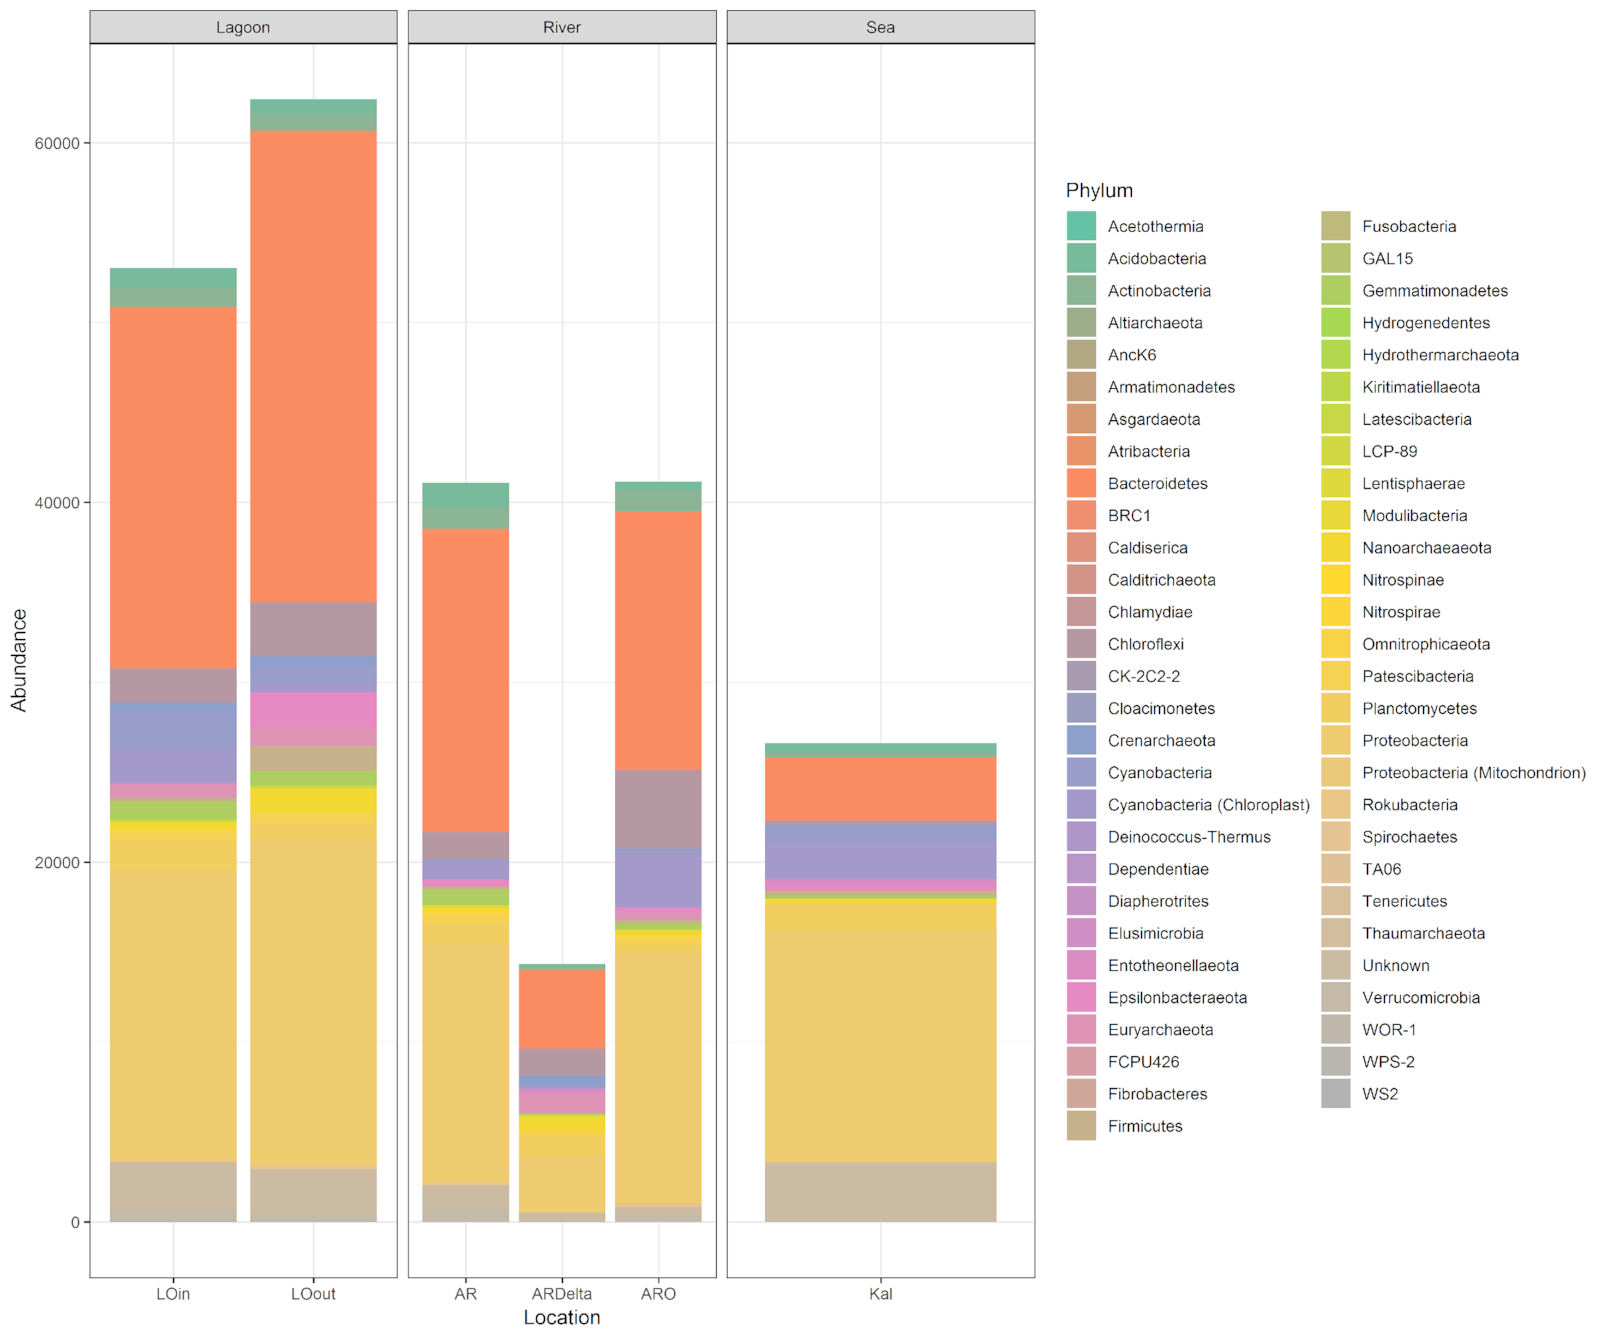
\includegraphics[width=105mm]{figures/giaa022fig3.jpeg}
         \caption[OTU bar plot at the phylum level.]{
            OTU bar plot at the phylum level. Bar plot depicting the taxonomy of the retrieved OTUs from PEMA for the dataset of Pavloudi et al. \citep{pavloudi2017sediment}, at the phylum level for the case of the 16S marker gene. AR: Arachthos; ARO: Arachthos Neochori; ARDelta: Arachthos Delta; LOin: Logarou station inside the lagoon; LOout: Logarou station in the channel connecting the lagoon to the gulf; Kal: Kalamitsi.
         }
         \label{fig:pema-barplot}
      \end{figure}


   \subsubsection*{COI marker gene analysis evaluation}

      Bista et al. \citep{bista2017annual} created 2 COI libraries of different sizes: COIS ($235$ - bp amplicon size) and COIF ($658$ - bp amplicon size). 
      The sequencing reads of COIS were selected for PEMA's evaluation; 
      the COIF sequencing read pairs had no overlap so as to be merged and therefore were not considered appropriate for the analysis.

      As previously, PEMA's performance was evaluated through a comparative analysis of the 
      Bista et al.~\citep{bista2017annual} dataset with 
      \href{https://github.com/enormandeau/barque}{Barque} 
      \footnote{
         \href{https://github.com/enormandeau/barque}{https://github.com/enormandeau/barque}
      }; 
      the commands and parameters chosen can be found in Additional File 1: Supplementary Methods. 
      Regarding the creation of the MOTU table, in the Bista et al. \citep{bista2017annual} study VSEARCH \citep{rognes2016vsearch} was used with a clustering at $97\%$ similarity threshold. 
      Afterwards, the BLAST+ (megablast) algorithm \citep{camacho2009blast} was used against a manually created database including all NCBI GenBank COI sequences of length $>100$  bp (June 2015) while excluding environmental sequences and higher taxonomic level information \citep{bista2017annual}. 
      As discussed in the publication, this approach resulted in $138$ unique MOTUs of which $73$ were assigned to species level. 
      For PEMA's evaluation, the chosen clustering algorithm was Swarm v2, using different options for the cluster radius ($d$) parameter (Table~\ref{table:pema-exec-times}); 
      according to Mahé et al. \citep{mahe2015swarm}, this is the most important parameter because it affects the number of MOTUs that are being created. 
      The resulting MOTUs were classified against the MIDORI reference database \citep{machida2017metazoan} using RDPClassifier \citep{wang2007naive}. 
      The results of the processing of the sequences are reported in Supplementary Table S3. 
      For the case of Barque, the BOLD Database was used \citep{ratnasingham2007bold}.


      % PEMA OUTPUT AND EXECUTION TIME
      \begin{table}[]
         \begin{center}    
            \begin{tabular}{@{}llllll@{}}
            \toprule
            \textbf{Parameter} & \textit{\textbf{d = 1}} & \textit{\textbf{d = 2}} & \textit{\textbf{d = 3}} & \textit{\textbf{d = 10}} & \textit{\textbf{d = 13}} \\ \midrule
            \begin{tabular}[c]{@{}l@{}}MOTUs after pre-process\\  and clustering steps\end{tabular} & 83,791 & 59,833 & 33,227 & 7,384 & 4,829 \\
            MOTUs after chimera removal & 80,347 & 57,863 & 32,539 & 7,339 & 4,796 \\
            Non-singleton MOTUs & 6,381 & 4,947 & 2,658 & 1,914 & 1,634 \\
            Assigned species & 62 & 83 & 86 & 86 & 84 \\
            Execution time (h) & 2:01:35 & 2:09:49 & 1:51:44 & 2:17:26 & 2:31:15 \\ \bottomrule
            \end{tabular}
            \caption[PEMA's output and execution time]{PEMA'sa output and execution time; PEMA's output and execution time (using a 20-core node) for different values of Swarm's d parameter.}
            \label{table:pema-exec-times}
         \end{center}
      \end{table}


      As shown in Table~\ref{table:pema-exec-times}, PEMA resulted in 83 species-level MOTUs with a cluster radius ($d$) of $2$, which is similar to the findings of the published study (i.e., $73$ species). 
      Although both the clustering algorithm and the taxonomy assignment methods were different between the original \citep{bista2017annual} and the present study, the results regarding the number of unique species present in the samples are in agreement to a considerable extent.

      The computational time required by PEMA for the completion of the analysis is also reported in Table~\ref{table:pema-exec-times}. 
      Regardless of the value of the d parameter, all analyses were completed in $∼2$ hours, i.e., fast enough to allow parameter testing and customization.
      Regarding Barque, the analysis resulted in the identification of $51$ species-level MOTUs and was concluded in $15$ minutes. 
      This difference is due to the error correction step of PEMA (BayesHammer algorithm \citep{nikolenko2013bayeshammer}), which plays an important part in the enhanced results that PEMA returns, but it also requires a certain computational time; 
      Barque does not have an analogous step, and therefore its overall execution time is shorter.
      
      PEMA performed better than Barque at identifying taxa that were included in the positive control contents of the published study (Table~\ref{table:pema-taxonomies-pema-barque}).

      % TABLE WITH SPECIES NAMES PEMA AND BARQUE
      \begin{table}[]
         \begin{tabular}{@{}lll@{}}
         \toprule

         \textbf{Barque} & \textbf{PEMA} & \textbf{Bista et al. {[}50{]}} \\ \midrule

         \textit{Ablabesmyia monilis*} & \textit{Ablabesmyia monilis*} & \textit{Ablabesmyia monilis} \\
         & \textit{Crangonyx pseudogracilis*} & \textit{Crangonyx pseudogracilis} \\
         & \textit{Radix sp.*} & \textit{Radix sp.} \\
         & Chironomidae sp.* & Chironomidae sp. \\
         & \textit{Ancylus sp.**} & \textit{Ancylus fluviatilis} \\
         & \textit{\begin{tabular}[c]{@{}l@{}}Athripsodes aterrimus, \\ Athripsodes cinereus**\end{tabular}} & \textit{Athripsodes albifrons} \\
         \textit{Chironomus anthracinus**} & \textit{\begin{tabular}[c]{@{}l@{}}Chironomus sp., \\ Chironomus anthracinus, \\ Chironomus pseudothummi,\\  Chironomus riparius**\end{tabular}} & \textit{Chironomus tentans} \\
         \textit{Polypedilum sordens**} &  & \textit{Polypedilum nubeculosum} \\
         \textit{Athripsodes aterrimus**} &  & \textit{Athripsodes albifrons} \\ \bottomrule
         \end{tabular}
         \caption[Comparing taxonomies retrieved from PEMA and Barque pipelines]{Comparison of the taxonomy of retrieved MOTUs among PEMA, Barque, and the positive controls of Bista et al. \citep{bista2017annual} ; * 
         Taxonomies identical to the published study (species level), ** Taxonomies identical to the published study (genus level).}
         \label{table:pema-taxonomies-pema-barque}
      \end{table}
      

   % PEMA DISCUSSION
   \subsection{Discussion}
   \label{sec:pema-discussion}

   \subsubsection*{OTU clustering vs ASV inference}
   \label{subsec:otu-asv}

      There is an ongoing discussion about whether ASVs exceed OTUs. 
      The strongest argument to this end is that ASVs are real biological sequences. 
      Hence, they can be compared between different studies in a straightforward way; 
      considered as consistent labels. 
      In comparison, de novo OTUs are constructed, or “clustered,” with respect to the emergent features of each specific dataset. 
      Therefore, OTUs defined in $2$ different datasets cannot be directly compared.

      However, the OTU concept is not compulsorily related to the clustering approach; 
      it is widely used to describe results based on its biological meaning but it does not imply clustering. 
      In addition, according to Callahan et al. \citep{callahan2017exact}, "ASV methods infer the biological sequences in the sample prior to the introduction of amplification and sequencing errors, and distinguish sequence variants differing by as little as one nucleotide." 
      As a result, ASVs could be considered as OTUs of higher resolution.

      It is due to this concept confusion that algorithms whose rationale is considerably closer to the variant-based approach are still considered as OTU clustering algorithms~\citep{callahan2017exact}. 
      Swarm v2 produces all possible \textit{microvariants} of an amplicon to implement an exact-string comparison~\citep{mahe2015swarm}. 
      Furthermore, real biological sequences, \textit{clouds of microvariants} are produced as its output, which can be used for comparisons between different studies. Thus, Swarm v2 can be considered as an ASV-inferring algorithm.

      Traditional clustering methods have certain limitations such as arbitrary global clustering thresholds and centroid selection because they depend on the input order and are time-consuming, etc.~\citep{mahe2014swarm}, which variant-based approaches manage to address. 
      However certain algorithms for OTU clustering such as VSEARCH have been proven to be especially reliable, and they are widely used by many researchers. 
      Furthermore, ASVs intend to improve taxonomic resolution; however, a vast number of inferred ASVs (see \href{http://fiererlab.org/2017/05/02/lumping-versus-splitting-is-it-time-for-microbial-ecologists-to-abandon-otus/}{here} 
      \footnote{
         \href{http://fiererlab.org/2017/05/02/lumping-versus-splitting-is-it-time-for-microbial-ecologists-to-abandon-otus/}{http://fiererlab.org/2017/05/02/lumping-versus-splitting-is-it-time-for-microbial-ecologists-to-abandon-otus/}
      } for more) can lead to inflation of diversity estimates, especially in the case of microbial communities, thus making the analysis even more complicated.

      ASV or OTU approaches are supported by PEMA, although we have found that similar ecological results are produced by both these methods, as also suggested by Glassman and Martiny~\citep{glassman2018broadscale}.


   \subsubsection*{Beyond environmental ecology, ongoing and future work}
   \label{subsec:pema-future}

      PEMA is mainly intended to support eDNA metabarcoding analysis and be directly applicable to next - generation biodiversity / ecological assessment studies. 
      Given that community composition analysis may also serve additional research fields, e.g., microbial pathology, the potential impact of such pipelines is expected to be much higher. 
      Ongoing PEMA work focuses on serving a wide scientific audience and on making it applicable to more types of studies. 
      The easy set - up and execution of PEMA allows users to work closely with national and European HPC / e - infrastructures (e.g., \href{https://www.elixir-greece.org/}{ELIXIR Greece} 
      \footnote{
         \href{https://www.elixir-greece.org/}{https://www.elixir-greece.org/}
      }, \href{https://www.lifewatch.eu/}{LifeWatch ERIC}, 
      \footnote{
         \href{https://www.elixir-greece.org/}{https://www.elixir-greece.org/}
      }
      \href{http://www.embrc.eu}{EMBRC ERIC} 
      \footnote{
         \href{http://www.embrc.eu}{http://www.embrc.eu}
      }
      ). 
      To that end and in a mid - term perspective, a CWL version of PEMA will be explored. 
      The aim of this effort is to reach out to a wider scientific audience and address both their ongoing as well as future analysis needs.

      By supporting the analysis of the most commonly used marker genes for Bacteria and Archaea (16S rRNA), Fungi (ITS), and Metazoa (COI/18S rRNA), a holistic biodiversity assessment approach is now possible through PEMA and eDNA metabarcoding; although, from a mid-term perspective, it is our intention to allow ad hoc and in - house databases to be used as reference for the taxonomy assignment.

   \subsubsection*{Conclusions}
   \label{subsec:pema-conclusion}

      PEMA is an accurate, execution - friendly and fast pipeline for eDNA metabarcoding analysis. 
      It provides a per - sample analysis output, different taxonomy assignment methods, and graphics - based biodiversity / ecological analysis. 
      This way, in addition to (M)OTU/ASV calling, it provides users with both an informative study overview and detailed result snapshots.

      Thanks to a nominal number of installation and execution commands required for PEMA to be set and run, it is considered essentially user friendly. 
      In addition, PEMA's strategic choice of a single parameter file, implementation programming language, and multiple container - type distribution grant it speed (running in parallel), on - demand partial pipeline enactment, and provision for HPC - system – based sharing.

      All the aforementioned features render PEMA attractive for biodiversity / ecological assessment analyses. 
      By supporting the analysis of the most commonly used marker genes for Prokaryotes (Bacteria and Archaea), as well as Eukaryotes (Fungi and Metazoa), PEMA allows assessment of biodiversity in different levels of biodiversity. 
      Applications may mainly concern environmental ecology, with possible extensions to such fields as microbial pathology and gut microbiome, in line with modern research needs, from low volume to big data.


   \subsection{Advances and PEMA modules added since its publication}

      PEMA has been under continuous development and testing.
      Custom databases can be now used to train both classifiers used in the PEMA framework, thus
      the taxonomy assignment step is not limited by the reference databases included on PEMA.
      With the release of the \href{https://github.com/hariszaf/pema/releases/tag/v.2.1.3}{v.2.1.3}
      \footnote{\href{https://github.com/hariszaf/pema/releases/tag/v.2.1.3}{https://github.com/hariszaf/pema/releases/tag/v.2.1.3}}
      version, PEMA was re-architectured completely aiming at an easier way for people to contribute. 
      On top of that, several modules have been added, mostly in an attempt to address requests from users and
      e-infrustructures (e.g., \href{https://www.lifewatch.eu/internal-joint-initiative/}{LifeWatch ERIC IJI}
      \footnote{\href{https://www.lifewatch.eu/internal-joint-initiative/}{https://www.lifewatch.eu/internal-joint-initiative/}}
      )(see Figure~\ref{fig:pema-lw}). 
      Similar efforts have been done so PEMA will be integrated in the 
      \href{https://hypatia.athenarc.gr/}{HYPATIA}
      \footnote{\href{https://hypatia.athenarc.gr/}{https://hypatia.athenarc.gr}}, 
      the Cloud infrastructure of the ELIXIR-GR community.


      \begin{figure}[h]
         \centering
         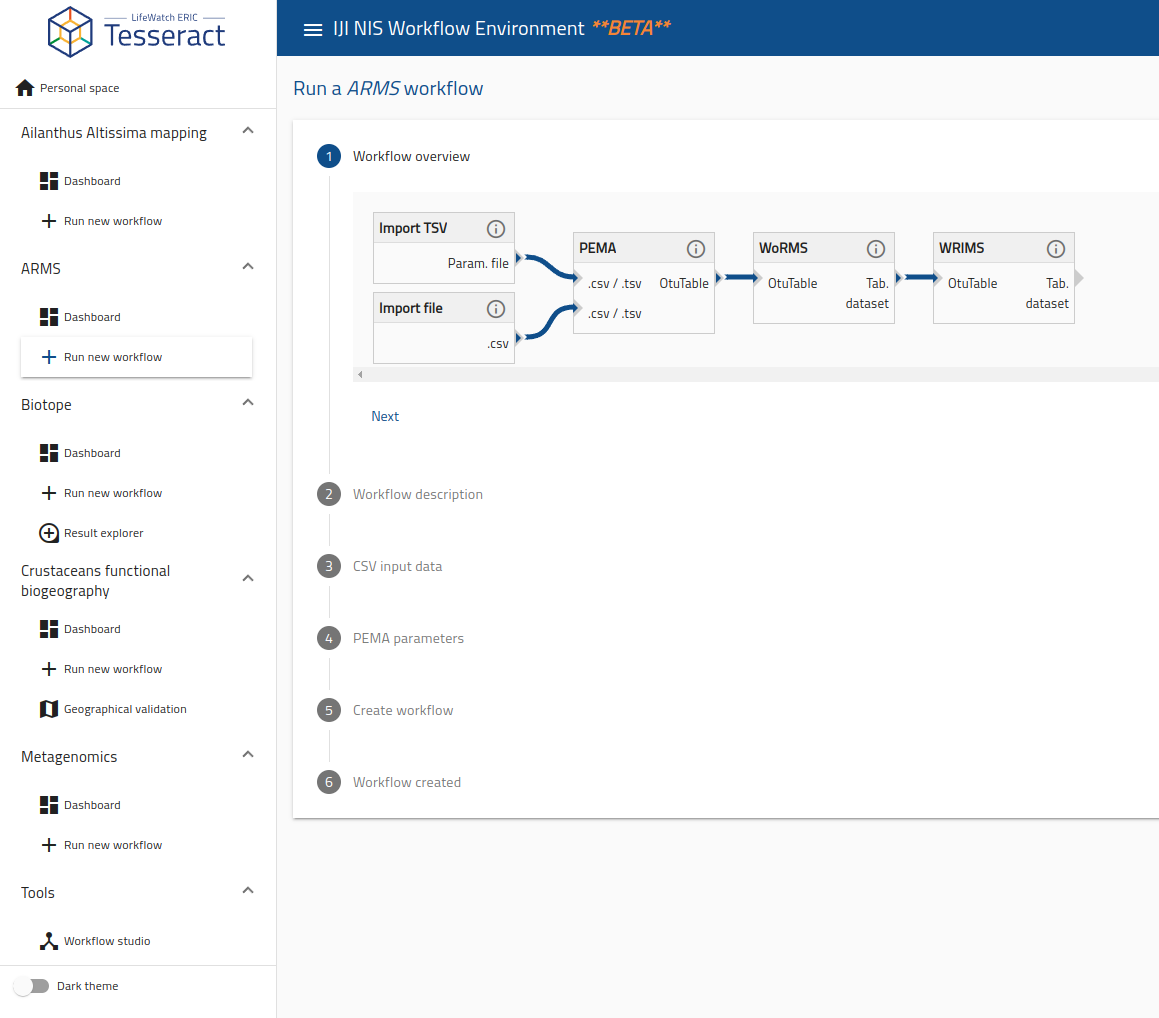
\includegraphics[width=0.95\columnwidth]{figures/pema_lw.png}
         \caption[PEMA at LifeWatch ERIC Tesseract portal]{
            PEMA is now available through the LifeWatch ERIC portal called Tesseract which is currently under a beta version. 
            A web interface is now available allowing users that are not familiar with Unix to use PEMA.
            Most importantly, users that have no access to computing resources required for their analyses
            can now use the capacity of Tesseract.  
         }
         \label{fig:pema-lw}
      \end{figure}

      On its current version (v.2.1.5) it now supports the analysis of one extra
      marker gene, the 12S rRNA gene, by exploiting the 12S Vertebrate Classifier v2.0.0-ref database \citep{teresita_m_porter_2021_5157047}.
      For the case of 18S rRNA marker gene, the PR2 database \citep{guillou2012protist} was integrated 
      so now the user may select between Silva and PR2,
      while Silva v.138 has been also added. 
      Furtheremore, thanks to the ncbi-taxonomist tool~\citep{buchmann2020collecting}, 
      PEMA now provides an extended OTU/ASV table where in the last column the NCBI Taxonomy Id 
      for the taxonomic level closer to the species name rank for which there is one, is available.
      Last but not least, a new version of the parameters file has been made to provide a machine-readable version 
      of it so the values set by the user can be parsed for potential errors in an automatic way. 

      The potential of the eDNA metabarcoding method as well as the 
      valid PEMA output
      were emphasized in a recent study where
      Autono-mous  Reef  Monitoring  Structures (ARMS) data 
      were combined with amplicon studies to 
      record, for the first time in Greek waters, the nudibranch 
      \textit{Anteaeolidiella lurana} (Ev. Marcus \& Er. Marcus, 1967)~\citep{bariche2020new}. 
   


      \subsection*{Supplementary Material}

      You may find the Supplementary files of this study through 
      \href{https://academic.oup.com/gigascience/article/9/3/giaa022/5803335#supplementary-data}{PEMA's publication}
      \footnote{\href{https://academic.oup.com/gigascience/article/9/3/giaa022/5803335\#supplementary-data}{https://academic.oup.com/gigascience/article/9/3/giaa022/5803335\#supplementary-data}}


      \textbf{Additional File 1:} Supplementary Methods: Description of tools invoked by PEMA and their licences. Description of the commands, along with their parameters, used to run PEMA, mothur, LotuS, and QIIME 2.

      \textbf{Additional File 2:} Mock Communities: Details about the mock communities chosen and their corresponding studies, as well as the returned output of PEMA for each for a number of sets of parameters.

      \textbf{Supplementary Table S1:} Number of sequences after each pre-processing step for the case of 16S rRNA gene.

      \textbf{Supplementary Table S3:} Number of sequences after each pre-processing step for the case of COI, dataset from Bista et al. \citep{bista2017annual}.

      \textbf{Supplementary Table S2:} Diversity indices of the samples.

      \textbf{Supplementary Figure S1:} Linear regression between the number of OTUs (averaged per sampling station) and the salinity of the sampling stations. L: Lagoon; S: Sea; R: River; AR: Arachthos; ARO: Arachthos Neochori; ARDelta: Arachthos Delta; LOin: Logarou station inside the lagoon; LOout: Logarou station in the channel connecting the lagoon to the gulf; Kal: Kalamitsi.

      \textbf{Supplementary Figure S2:} Bar plot depicting the taxonomy of the retrieved OTUs from LotuS at the phylum level.

      \textbf{Supplementary Figure S3:} Bar plot depicting the taxonomy of the retrieved OTUs from QIIME 2 using Deblur at the phylum level.

      \textbf{Supplementary Figure S4:} Bar plot depicting the taxonomy of the retrieved OTUs from QIIME 2 using DADA2 at the phylum level.

      \textbf{Supplementary Figure S5:} Bar plot depicting the taxonomy of the retrieved OTUs from LotuS at the class of Betaproteobacteriales.

      \textbf{Supplementary Figure S6:} Bar plot depicting the taxonomy of the retrieved OTUs from QIIME 2 using Deblur at the class of Betaproteobacteriales.

      \textbf{Supplementary Figure S7:} Bar plot depicting the taxonomy of the retrieved OTUs from PEMA at the class of Betaproteobacteriales.




   \newpage


% ----------------------------------------
% 
%      DARN
% 
% ----------------------------------------

\newpage

% SECTION 3
\section[The Dark mAtteR iNvestigator (DARN) tool: getting to know the known unknowns in COI amplicon data]{
      The Dark mAtteR iNvestigator (DARN) tool: getting to know the known unknowns in COI amplicon data\footnote{
      For author contributions and supplementary material please refer to the relevant sections. 
      % Modified version of the published review.
   }
}
\label{publ:darn}

\textbf{Citation:} \\
Zafeiropoulos, H., Gargan, L., Hintikka, S., Pavloudi, C. and Carlsson, J., 2021. The Dark mAtteR iNvestigator (DARN) tool: getting to know the known unknowns in COI amplicon data. Metabarcoding and Metagenomics, 5, p.e69657, \\
DOI: \href{https://doi.org/10.3897/mbmg.5.69657}{10.3897/mbmg.5.69657}

   \subsection{Abstract}
   The mitochondrial cytochrome C oxidase subunit I gene (COI) is commonly used in environmental DNA (eDNA) metabarcoding studies, especially for assessing metazoan diversity. 
   Yet, a great number of COI operational taxonomic units (OTUs) or/and amplicon sequence variants (ASVs) retrieved from such studies do not get a taxonomic assignment with a reference sequence. 
   To assess and investigate such sequences, we have developed the Dark mAtteR iNvestigator (DARN) software tool. For this purpose, a reference COI-oriented phylogenetic tree was built from $1,593$ consensus sequences covering all the three domains of life. 
   With respect to eukaryotes, consensus sequences at the family level were constructed from 183,330 sequences retrieved from the Midori reference 2 database, which represented $70\%$ of the initial number of reference sequences. 
   Similarly, sequences from $431$ bacterial and $15$ archaeal taxa at the family level ($29\%$ and $1\%$ of the initial number of reference sequences respectively) were retrieved from the BOLD and the PFam databases. 
   DARN makes use of this phylogenetic tree to investigate COI pre-processed sequences of amplicon samples to provide both a tabular and a graphical overview of their phylogenetic assignments. 
   To evaluate DARN, both environmental and bulk metabarcoding samples from different aquatic environments using various primer sets were analysed. 
   We demonstrate that a large proportion of non-target prokaryotic organisms, such as bacteria and archaea, are also amplified in eDNA samples and we suggest prokaryotic COI sequences to be included in the reference databases used for the taxonomy assignment to allow for further analyses of dark matter. 
   DARN source code is available on GitHub at \href{https://github.com/hariszaf/darn}{https://github.com/hariszaf/darn} and as a Docker image at \href{https://hub.docker.com/r/hariszaf/darn}{https://hub.docker.com/r/hariszaf/darn}.

   \subsection{Introduction}
   \label{sec:darn-intro}

   % Parts of the following need to be moved in the main Intro
   \subsubsection*{Metabarcoding: concept and caveats}
   \label{subsec:darn-intro-metabar}

   DNA metabarcoding is a rapidly evolving method that is being more frequently employed i
   n a range of fields, such as biodiversity, biomonitoring, molecular ecology and others 
   \citep{deiner2017environmental, ruppert2019past}. 
   Environmental DNA (eDNA) metabarcoding, targeting DNA directly isolated from environmental samples
   (e.g., water, soil or sediment, \citep{taberlet_environmental_2012}), is considered a holistic approach 
   (Stat et al. 2017) in terms of biodiversity assessment, providing high detection capacity. 
   At the same time, it allows wide-scale rapid bio-assessment \citep{stat2017ecosystem} at a relatively
   low cost as compared to traditional biodiversity survey methods \citep{ji2013reliable}.

   The underlying idea of the method is to take advantage of genetic markers, i.e. marker loci, 
   using primers anchored in conserved regions. 
   These universal markers should have enough sequence variability to allow distinction among 
   related taxa and be flanked by conserved regions allowing for universal or semi-universal primer design \citep{deagle2014dna}. 
   In the case of eukaryotes, the target is most commonly mitochondrial due to higher copy numbers than nuclear DNA and the potential for species level identification. 
   Furthermore, mitochondria are nearly universally present in eukaryotic organisms, especially in case of metazoa, and can be easily sequenced and used for identification of the species composition of a sample \citep{taberlet2012towards}. 
   However, it is essential that comprehensive public databases containing well curated, up-to-date sequences from voucher specimens are available \citep{schenekar2020reference}. 
   This way, sequences generated by universal primers can be compared with the ones in reference databases, assessing sample OTU composition. 
   The taxonomy assignment step of the eDNA metabarcoding method and thus, the identification via DNA-barcoding, is only as good and accurate as the reference databases \citep{cilleros2019unlocking}. 

   Nevertheless, there is not a truly “universal” genetic marker that is capable of being amplified for all species across different taxa \citep{kress2015dna}. 
   Different markers have been used for different taxonomic groups \citep{deiner2017environmental}. 
   While bacterial and archaeal diversity is often based on the 16S rRNA gene, for eukaryotes a diverse set of loci is used from the analogous eukaryotic rRNA gene array (e.g., ITS, 18S or 28S rRNA), chloroplast genes (for plants) and mitochondrial DNA (for eukaryotes) in an attempt for species - specific resolution \citep{coissac2012bioinformatic}. 
   The mitochondrial cytochrome c oxidase subunit I (COI) marker gene has been widely used for the barcoding of the Animalia kingdom for almost two decades \citep{hebert2003barcoding}.
   There are cases where COI has been the standard marker for metabarcoding, such as in the assessment of freshwater macroinvertebrates \citep{elbrecht2017validation} even though not all taxonomic groups can be differentiated to the species level using this locus \citep{deiner2017environmental}; 
   for example, in case of fish other loci are widely used such as 12S rRNA gene (hereafter referred to as 12S rRNA) \citep{miya2020mifish}.

   \subsubsection*{The COI locus}
   \label{subsec:darn-intro-coi}

   The mitochondrial cytochrome c oxidase subunit I (also called cox1 or/and COI) is a gene fragment of ~700 bp, widely used for metazoan diversity assessment. Here we present some of the reasons that microbial eukaryotes and prokaryotes are also amplified in such studies, raising the issue of the known unknown sequences.
   COI is a fundamental part of the heme aa3-type mitochondrial cytochrome c oxidase complex: the terminal electron acceptor in the respiratory chain. 
   Even if aa3-type Cox have been found in bacteria, there are also other cytochrome c oxidase (Cox) groups, such as the cbb3-type cytochrome c oxidases (cbb3-Cox) and the cytochrome ba3 \citep{ekici2012biogenesis, schimo2017cytochrome}.

   Furthermore, the presence of highly divergent nuclear mitochondrial pseudogenes (numts) has been a widely known issue on the use of COI in barcoding and metabarcoding studies, leading to overestimates of the number of taxa present in a sample \citep{song2008many}.
   Numts are nonfunctional copies of mtDNA in the nucleus that have been found in major clades of eukaryotic organisms \citep{bensasson2001mitochondrial}.

   Thus, as Mioduchowska et al. (2018) \citep{mioduchowska2018instances} highlight, when universal primers are used targeting the COI locus, it is possible to co-amplify both non-target numts and prokaryotes \citep{siddall2009barcoding}. This has led to multiple erroneous DNA barcoding cases and it is now not rare to encounter bacterial sequences described as metazoan in databases such as GenBank \citep{mioduchowska2018instances}.

   Even though there are various known issues \citep{deagle2014dna}, COI is indeed considered as the “gold standard” for community DNA metabarcoding of bulk metazoan samples \citep{andujar2018coi}; 
   bulk is an environmental sample containing mainly organisms from the taxonomic group under study providing high quality and quantity of DNA \citep{taberletanalysis}. 
   However, as highlighted in the same study, this is not the case for eDNA samples. 
   As Stat et al. (2017) \citep{stat2017ecosystem} state, in the case of eDNA samples, the target region for metazoa is found in general at considerably lower concentrations compared to those from prokaryotes because most primers targeting the COI region amplify large proportions of prokaryotes at the same time \citep{yang2013testing, yang2014using, collins2019non}. 
   Cold-adapted marine gammaproteobacteria are an indicative example for this case as shown by Siddall et al. (2009) \citep{siddall2009barcoding}.



% DARN CONTRIBUTION
   \subsection{Contribution}
   \label{sec:darn-contribution}

   The co-amplification of prokaryotes explained above, is a major reason for why many Operational Taxonomic Units (OTUs) and/or Amplicon Sequence Variants (ASVs) in eDNA metabarcoding studies cannot get taxonomy assignments when metazoan reference databases are used (c.f. Aylagas et al. 2016 \citep{aylagas2016benchmarking}) or they are assigned to metazoan taxa but with very low confidence estimates. 
   Despite the presence of such OTUs/ASVs to a varying degree in metabarcoding studies using the COI marker gene \citep{siddall2009barcoding}, to the best of our knowledge, there has not been a thorough investigation of the origin for these sequences. 
   Although unassignable sequences could be informative, there have been few attempts to further investigate this dark matter (e.g., \citep{sinniger2016worldwide, haenel2017ngs}).
   
   The aim of this study was to build a framework for extracting such non-target, potentially unassigned (or assigned with low confidence) sequences from COI environmental sequence samples, hereafter referred to as “dark matter” as per Bernard et al. (2018) \citep{bernard2018microbial}. 
   We argue that the vast majority of these sequences represent microbial taxa, such as bacteria and archaea. 
   
   More specifically, based on the previously described methodology by Barbera et al. (2019) \citep{barbera2019epa} (see also full stack example of the EPA-ng algorithm) for large-scale phylogenetic placements, we built a framework to estimate to what extent the OTUs/ASVs retrieved in an environmental sample represent target taxa or not. 
   That is, to evaluate the taxonomy assignment step in a metabarcoding analysis, by checking the phylogenetic placement of dark matter sequences. Similar studies have provided great insight into other marker genes, e.g. \citep{jamy2020long}.


% DARN METHODS
   \subsection{Methods \& Implementation}
   \label{sec:darn-methods}

   \subsubsection*{Building the COI tree of life}
   \label{subsec:darn-methods-tree}

   Sequences for the COI region from all the three domains of life were retrieved from curated databases. 
   Eukaryotic sequences were retrieved from the Midori reference 2 database (version: GB239) \citep{machida2017metazoan}. 
   Initially, $1,315,378$ sequences were retrieved corresponding to $183,330$ unique species from all eukaryotic taxa. 
   With respect to bacteria and archaea, $3,917$ bacterial COI sequences were obtained from the BOLD database \citep{ratnasingham2007bold}. 
   Similarly, $117$ sequences from archaea were obtained from BOLD. 
   In addition, for all the PFam protein sequences related to the accession number for 
   COX1 (\href{http://www.ncbi.nlm.nih.gov/nuccore/PF00115}{PF00115}
      \footnote{
         \href{http://www.ncbi.nlm.nih.gov/nuccore/PF00115}{http://www.ncbi.nlm.nih.gov/nuccore/PF00115}
      }
   ), the respective DNA sequences were extracted from their corresponding genomes. 
   This way an additional $217$ archaeal and $9,154$ bacterial sequences were obtained (see Table 1). 
   In total, sequences from $15$ archaeal, $371$ bacterial families and 60 taxonomic groups of higher level not assigned in the family level, were gathered. 
   An overview of the approach that was followed is presented in Figure~\ref{fig:darn-build-tree}. 

   The large number of obtained sequences effectively prevents a phylogenetic tree construction encompassing their total number in terms of building a single phylogenetic tree covering all of the three domains of life (archaea, bacteria, eukaryota). 
   Therefore, consensus representative sequences from each of the three datasets were constructed using 
   the PhAT algorithm \citep{czech2019methods}; 
   based on the entropy of a set of sequences, PhAT groups sequences into a given target number of groups so they reflect the diversity of all the sequences in the dataset. 
   As PhAT uses a multiple sequence alignment (MSA) as input, all the three domain-specific datasets were aligned using the MAFFT alignment software tool v7.453 \citep{katoh2002mafft, nakamura2018parallelization}.
   
   % Table with sequences numbers
   \begin{table}[h]
      \begin{tabular}{@{}lllll@{}}
      \toprule
      \multirow{2}{*}{\textbf{Resources}} & \multicolumn{2}{l}{\textbf{bacteria}} & \multicolumn{2}{l}{\textbf{archaea}} \\ \cmidrule(l){2-5} 
      & \textbf{\# of sequences} & \textbf{\# of strains} & \textbf{\# of sequences} & \textbf{\# of strains} \\ \cmidrule(r){1-1}
      BOLD & 3,917 & 2,267 & 117 & 117 \\
      PFam-oriented & 9,154 & 4,532 & 217 & 115 \\ \bottomrule
      \end{tabular}
      \caption[Number of sequences and taxonomic species per domain of life and resources]{Number of sequences and taxonomic species per domain of life and resources. The (\#) symbols stands for "number".}
      \label{table:darn-seq-per-domain}
   \end{table}


   In the case of Eukaryotes, the alignment of the corresponding sequences would be impractically long because of their large number ($~183$K sequences). 
   To address this challenge, a two-step procedure was followed; 
   a sequence subset of $500$ sequences (\textit{reference set}) was selected and aligned and then used as a backbone for the alignment of all the remaining eukaryotic COI sequences. 
   All sequences were considered reliable as they were retrieved from curated databases (Midori2 and BOLD). 
   To build the reference set, a number ($n$) of the longest sequences from each of the various phyla were chosen, proportionally to the number ($m$) of sequences of each phylum (see Supplementary Table~\ref{table:darn-seq-per-domain}). 
   The \texttt{--min-tax-level} parameter of the PhAT algorithm corresponded to the class level, for the case of eukaryotes and to the family level for archaea and bacteria. 
   This parameter forced the PhAT algorithm to build at least one consensus sequence for each class and family respectively. 
   The taxonomy level was not the same for the case of eukaryotes sequence dataset and those of bacteria and archaea, as the number of unique eukaryotic families was one order of magnitude higher. 
   The PhAT algorithm was invoked through the gappa v0.6.1 collection of algorithms \citep{czech2020genesis}.


   % Figure with the DARN methodology steps
   \begin{figure}
      \centering
      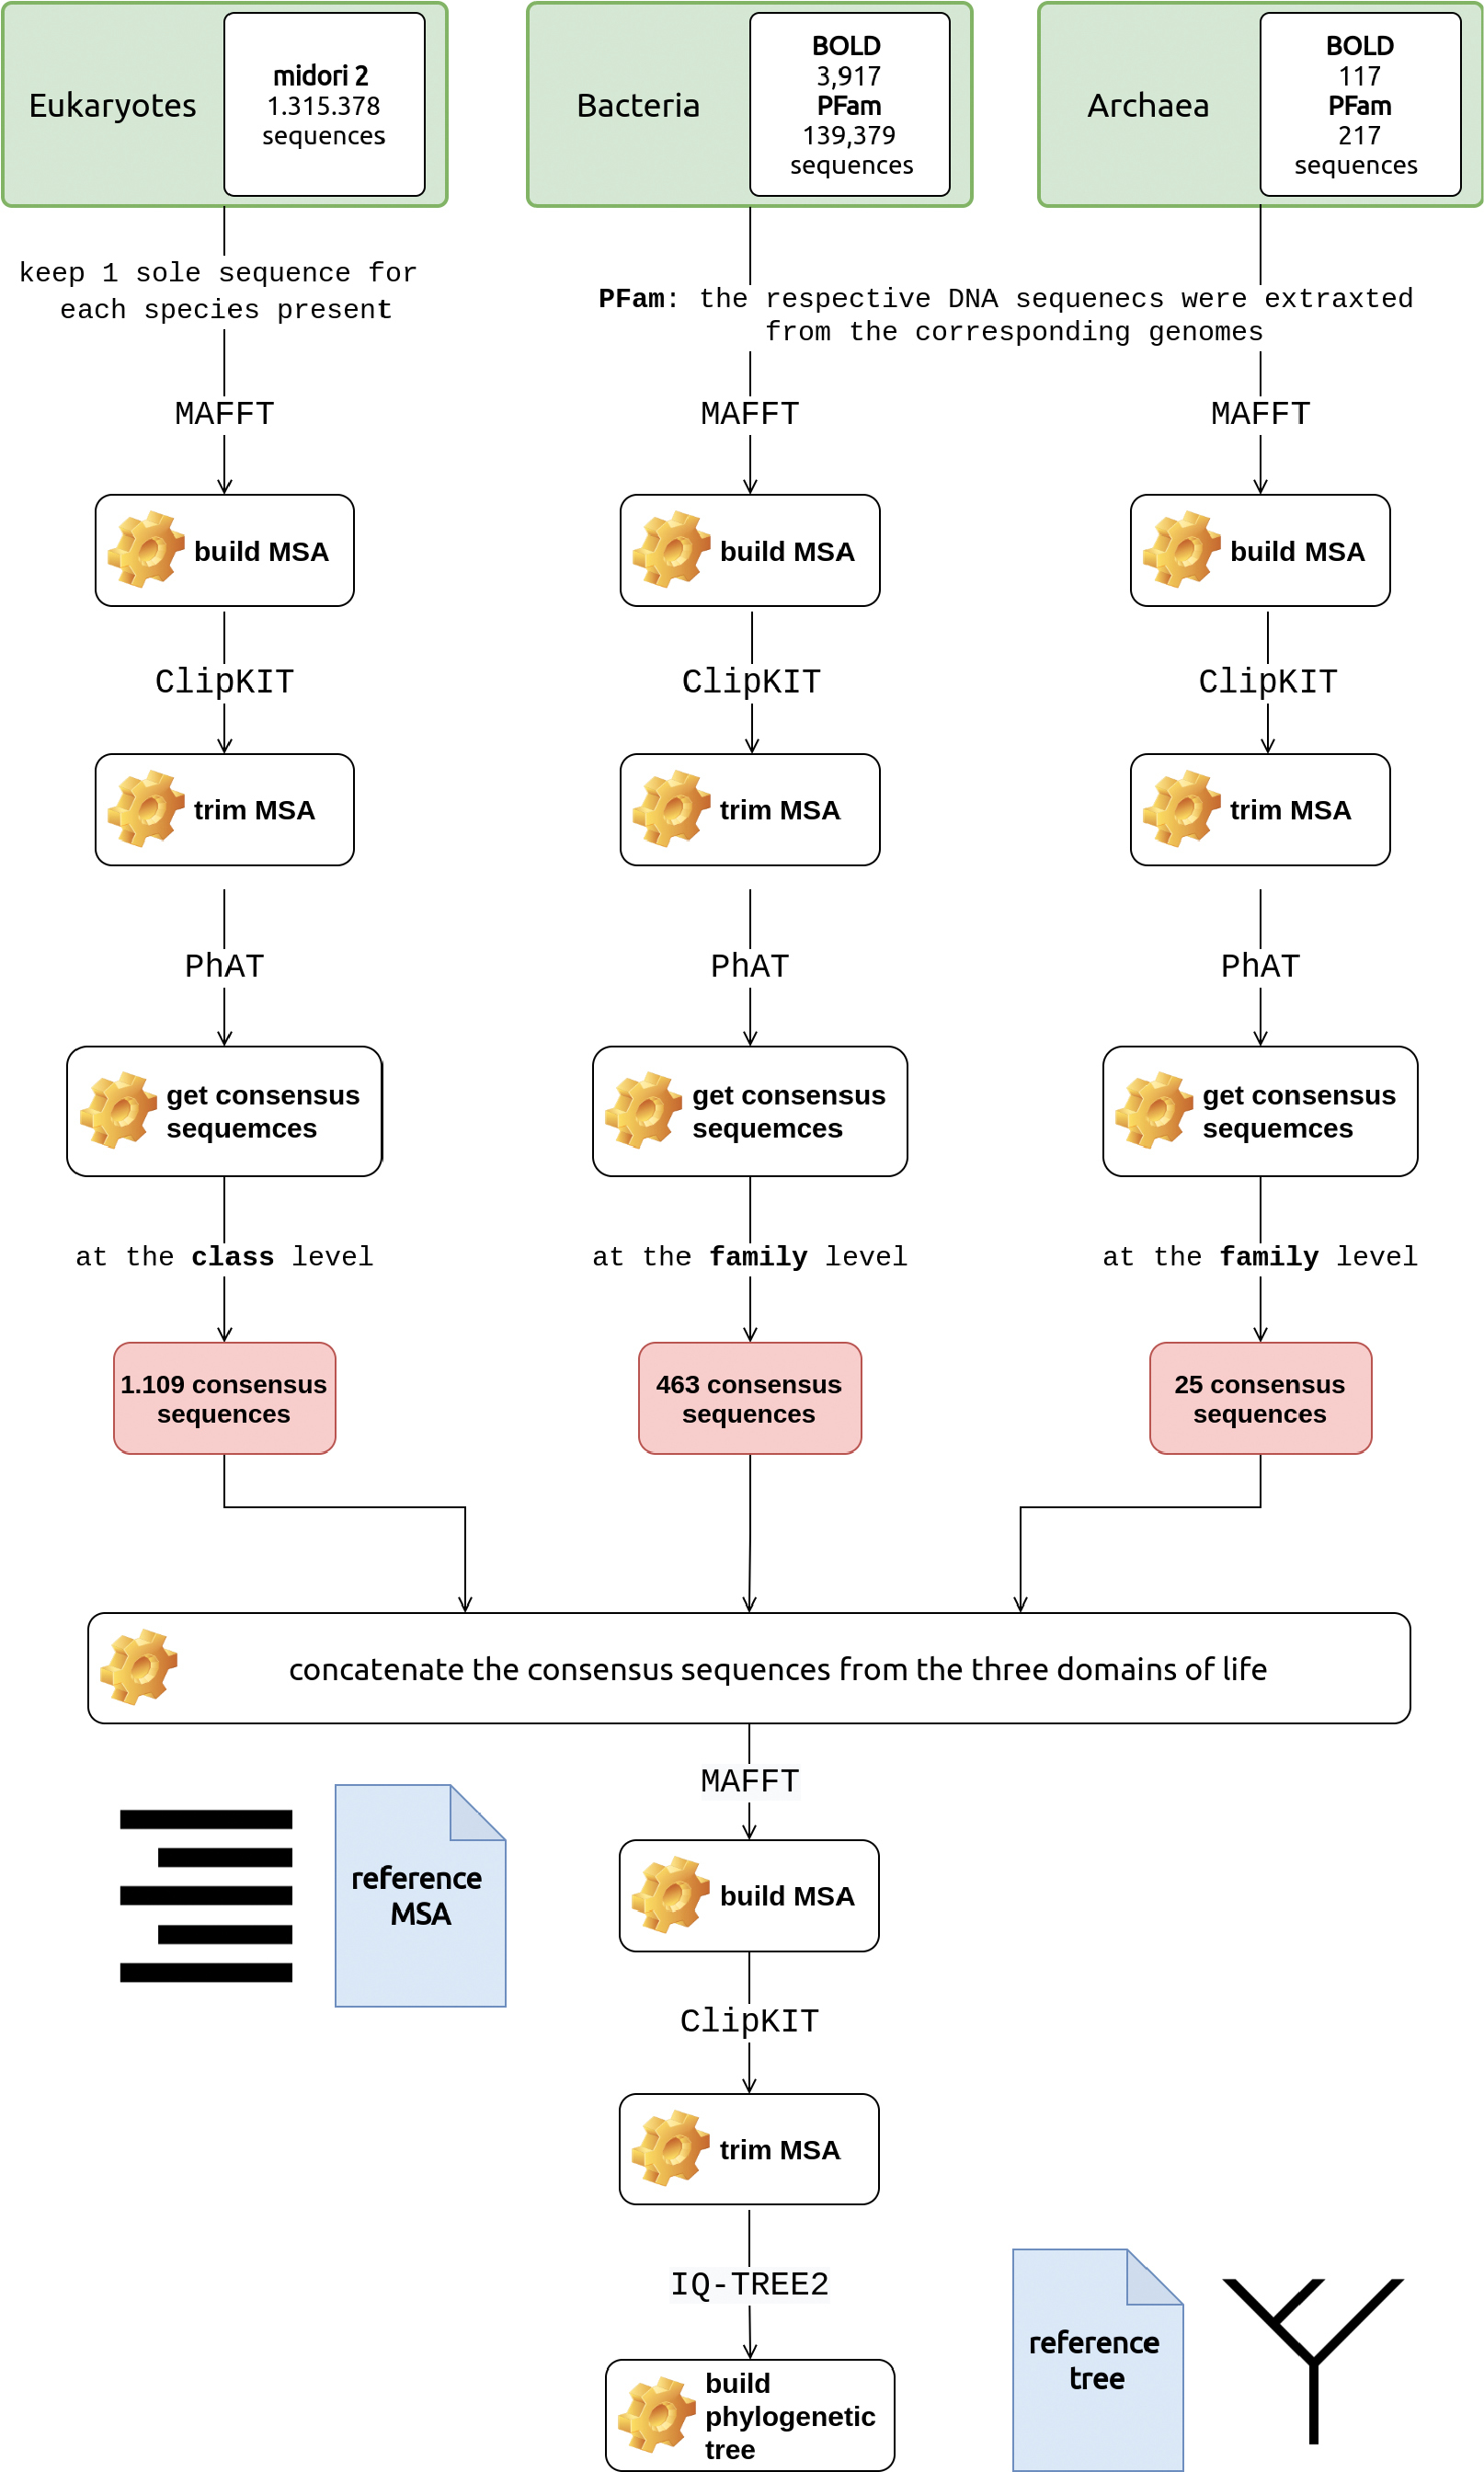
\includegraphics[width=100mm]{figures/darn_methodology.jpg}
      \caption[Building the COI reference tree of life]{
         Overview of the approach followed to build the COI reference tree of life. 
         Sequences were retrieved from Midori 2 (eukaryotes) and BOLD (bacteria and archaea) repositories. 
         Consensus sequences at the family level were built for each domain specific dataset. 
         MAFFT and consensus sequences at the family level were built using the PhAT algorithm. 
         The COI reference tree was finally built using IQ-TREE2. 
         Noun project icons by Arthur Slain and A. Beale.
      }
      \label{fig:darn-build-tree}
   \end{figure}


   A total of $1,109$ consensus sequences ($70\%$ of total consensus sequences) were built covering the eukaryotic taxa, 
   while $463$ ($29\%$) bacterial and $21$ ($1\%$) archaeal consensus sequences were included. 
   The per-domain, consensus sequences returned can be found under the \texttt{consensus\_seqs} directory on 
   the GitHub repository 
   (see \texttt{\_consensus.fasta} files). 
   These sequences were then merged as a single dataset and aligned to build a reference MSA; 
   this time MAFFT was set to return using the \texttt{--globalpair} algorithm and the \texttt{--maxiterate} parameter 
   equal to $1,000$. 
   The MSA returned was then trimmed with the ClipKIT software package \citep{steenwyk_clipkit_2020} to keep only phylogenetically informative sites. 
   The final MSA is available on GitHub; \\
   see the \href{https://github.com/hariszaf/coi_dark_matter/blob/6df8559f27165f5327e4e56e9c36f5fab291fe49/build_tree_of_life/consensus_seqs/trimmed_all_consensus_aligned_adjust_dir.aln}{\texttt{trimmed\_all\_consensus\_aligned\_adjust\_dir.aln}} file.

   The reference tree was then built based on this trimmed MSA using the IQ-TREE2 software \citep{hoang2018ufboot2, minh_iq-tree_2020}.
   ModelFinder was invoked through IQ-TREE2 and the \texttt{GTR+F+R10} model was chosen based on the 
   Bayesian Information Criterion (BIC) among $286$ models that were tested. 
   The phylogenetic tree was then built using $1,000$ bootstrap replicates (\texttt{-B} $1,000$) and 
   $1,000$ bootstrap replicates for Shimodaira–Hasegawa-like approximate likelihood ratio test (SH-aLRT) (\texttt{1,000} $1000$).
   
   In the \texttt{.iqtree} file there are the branch support values; SH-aLRT support (\%) / ultrafast bootstrap support (\%).
   
   A thorough description of all the implementation steps for building the reference tree is presented in this 
   \href{https://colab.research.google.com/drive/1XorHsBm1uqx5TTZsH7SeVRkUA2SS8dnY}{Google Collab Notebook} 
   \footnote{
      \href{https://colab.research.google.com/drive/1XorHsBm1uqx5TTZsH7SeVRkUA2SS8dnY}{https://colab.research.google.com/drive/1XorHsBm1uqx5TTZsH7SeVRkUA2SS8dnY}
   }
   . 
   The computational resources of the IMBBC High Performance Computing system, called Zorba \citep{zafeiropoulos_0s_2021}, were exploited to address the needs of the tasks.


   \subsubsection*{Investigating COI dark matter}
   \label{subsec:darn-methods-investigate}

   The COI reference tree was subsequently used to build and implement the Dark mAtteR iNvestigator (DARN) software tool. 
   DARN uses a \texttt{.fasta} file with DNA sequences as input and returns an overview of sequence assignments per domain (eukaryotes, bacteria, archaea) after placing the query sequences of the sample on the branches of the reference tree. 
   Sequences that are not assigned to a domain are grouped as "distant". 
   It is necessary for the input sequences to represent the proper strand of the locus, 
   i.e. input reads should have forward orientation. 
   Optionally, DARN invokes the orient module of the vsearch package \citep{rognes2016vsearch} to implement this step, in case the user is not sure about the orientation of the sequences to be analysed.

   The focal query sequences are aligned with respect to the reference MSA using the PaPaRa 2.0 algorithm \citep{berger2012papara}. 
   The query sequences are then split to build a discrete query MSA. 
   Finally, the Evolutionary Placement Algorithm EPA-ng \citep{barbera2019epa} is used to assign the query sequences to the reference tree.

   To visualise the query sequence assignments, a two-step method was developed. 
   First, DARN invokes the gappa examine assign tool which taxonomically assigns placed query sequences by making use of the likelihood weight ratio (LWR) that was assigned to this exact taxonomic path. 
   In the DARN framework, by making use of the \texttt{--per-query-results} and \texttt{--best-hit} flags, the gappa assign software assigns the LWR of each placement of the query sequences to a taxonomic rank that was built based on the taxonomies included in the reference tree. 
   The first flag ensures that the gappa assign tool will return a tabular file containing one assignment profile per input query while the latter will only return the assignment with the highest LWR. 
   DARN automatically parses this output of gappa assign to build two input Krona profile files based on 

   \begin{itemize}
      \item the LWR values of each query sequence and
      \item an adjustive approach where all the best hits get the same value in a binary approach (presence - absence)
   \end{itemize}
   
   In the \texttt{final\_outcome} directory that DARN creates, two \texttt{.html} files, one for each of the Krona plots; 
   Krona plots are built using the ktImportText command of KronaTools \citep{ondov2011interactive}. 
   In addition four \texttt{.fasta} files are generated including the sequences of the sample that have been assigned to each domain or as "distant". 
   A \texttt{.json} file with the metadata of the analysis is also returned including the identities of the sequences assigned to each domain.

   DARN also runs the gappa assign tool with the \texttt{--per-query-results} flag only. 
   This way, the user can have a thorough overview of each sample’s sequence assignments, as a sequence may be assigned to more than one branch of the reference tree, sometimes even to different domains. 
   However, in cases with sequences assigned to multiple branches, the likelihood scores are most typically up to 100-fold to 1000-fold different.

   DARN source code as well as all data sequences and scripts for building the reference phylogenetic tree are available on \href{https://github.com/hariszaf/darn}{GitHub} \footnote{
      \href{https://github.com/hariszaf/darn}{https://github.com/hariszaf/darn}
   }.



% DARN RESULTS
   \subsection{Results \& Validation}
   \label{darn-results}
   \subsubsection*{Evaluation of the phylogenetic tree}
   \label{darn-results-tree-evaluation}

   The inferred phylogenetic tree is shown in Figure~\ref{fig:darn-ref-placements}, with the bacterial (light blue) and archaeal (dark green) branches highlighted;
   in Supplementary material 3: Figure S1 the distribution of the eukaryotic phyla on the tree is presented. 
   As shown, bacteria and archaea can be distinguished from eukaryotes. 
   Scattered bacterial branches that are present among eukaryotic ones represent the diversity of the COI locus. 
   To evaluate the phylogenetic tree, the set of consensus sequences were placed on it using the EPA-ng algorithm. 
   The placements (see \texttt{.jplace} through a phylogenetic tree viewer, e.g. iTOL) verified that the phylogenetic tree built is valid, as the consensus sequences have been placed in their corresponding taxonomic branches (Supplementary material 4: Figure S2; the figure was built using the heat-tree module of the gappa examine tool).

   % FIGURE WITH PLACEMENTS
   \begin{figure}[h]
      \centering
      \includegraphics[width=135mm]{figures/placements_of_consensus_seqs_transpaernt.png}
      \caption[Placements of the consensus COI sequences on the reference COI tree]{
         Phylogenetic tree of the consensus sequences retrieved; the tree that DARN makes use of. Light blue: bacterial branches. 
         Dark green: archaeal branches. White: eukaryotic branches.
      }
      \label{fig:darn-ref-placements}
   \end{figure}


   \newpage

   \subsubsection*{DARN using mock community data}

   To examine whether the phylogenetic-based taxonomy assignment addresses a real-world issue, a local blast database was built using the total number of the consensus sequences retrieved. 
   As expected, when the consensus sequences were blasted against this local blastdb, all were matched with their corresponding sequences. 
   However, when a mock dataset was used to evaluate the two approaches (\texttt{blastdb} and the phylogenetic tree) none of the bacterial sequences were captured as bacteria after \texttt{blastn} against the local blastdb (see output file \href{https://github.com/hariszaf/darn/blob/pfam/evaluation/consensus_blast_assignments.txt}{here} 
   \footnote{
      \href{https://github.com/hariszaf/darn/blob/pfam/evaluation/consensus_blast_assignments.txt}{https://github.com/hariszaf/darn/blob/pfam/evaluation/consensus\_blast\_assignments.txt}
   }). 
   All bacterial sequences returned an incorrect eukaryotic assignment. 
   Contrarily, when the phylogenetic tree was used, all the bacterial sequences were captured.


   \subsubsection*{DARN using real community data}

   To evaluate DARN on the presence of dark matter we analysed a wide range of cases to show the ability of DARN to detect and estimate dark matter under various conditions. 
   Both eDNA and bulk samples, from marine, lotic and lentic environments, were selected to reflect various combinations of primer and amplicon lengths, PCR protocols and bioinformatics analyses (Table~\ref{table:darn-samples-outcomes}).

   % BIG TABLE WITH DARN OUTPUT TABLES
   \begin{sidewaystable}
      
      \begin{tabular}{@{}cccccccccc@{}}
      
      \toprule

      % HEAD LINE 1 
      \multirow{2}{*}{\begin{tabular}[c]{@{}c@{}}Sample(s) \\ accession number\end{tabular}} & 
         \multirow{2}{*}{Sample type} & 
         \multirow{2}{*}{Primer set} & 
         \multirow{2}{*}{\begin{tabular}[c]{@{}c@{}}Amplicon \\ length (bp)\end{tabular}} & 
         \multirow{2}{*}{\begin{tabular}[c]{@{}c@{}}Bioinfo \\ pipeline(s)\end{tabular}} & 
         \multirow{2}{*}{\# of ASVs} & \multicolumn{4}{c}{\begin{tabular}[c]{@{}c@{}}$\sim$\% of sequence assignments per domain \\ (if PEMA\footnote{The $d$ parameter equals $10$ except mentioned otherwise})\end{tabular}} \\ \cmidrule(l){7-10} 
      
      % HEAD LINE 2 - DOMAINS 
      &  &  &  &  &  & \multicolumn{1}{c|}{Eukaryotes} & 
         \multicolumn{1}{c|}{Bacteria} & 
         \multicolumn{1}{c|}{Archaea} & 
         \multicolumn{1}{c|}{distant} \\ \midrule

      % LINE 1
      \multirow{4}{*}{
         \begin{tabular}[c]{c@{}c@{}}
            ERS6449795- \\ ERS6449829 
         \end{tabular}
      } & 
      
      \multirow{4}{*}{eDNA} & 

      \multirow{4}{*}{
         \begin{tabular}[c]{c@{}c@{}c@{}c@{}}
            jgHCO2198 - \\ jgLCO1490 \& \\ LoboF1 - \\ LoboR1
         \end{tabular}
      } & 

      \multirow{4}{*}{658} & 

      \multirow{4}{*}{
         \begin{tabular}[c]{c@{}c@{}}
            QIIME2 - \\ Dada2 \\ PEMA \\ &
         \end{tabular} 

      } & 13,376 & 11 & 88.0 & 0.02 & 0.003 \\ & & & & \\
      
      % \multirow{2}{*}{ 
         % \begin{tabular}[c]{c@{}c@{}}
         %    PEMA
         % \end{tabular} 
      % } 
      & & & & & 39,454 & 25 & 75.0 & 0.1 & 0.4 \\  
         
      \\
      \midrule

      % LINE 2
      \multirow{6}{*}{\begin{tabular}[c]{@{}c@{}}ERS6463899–\\ ERS6463901\end{tabular}} & \multirow{15}{*}{eDNA} & \multirow{15}{*}{\begin{tabular}[c]{@{}c@{}}mlCOIintF - \\ jgHCO2198\end{tabular}} & \multirow{15}{*}{313} & JAMP & \multirow{5}{*}{1,304} & \multirow{5}{*}{35} & \multirow{5}{*}{65.0} & \multirow{5}{*}{-} & \multirow{5}{*}{0.2} \\

      &  &  &  & dada2 &  &  &  &  &  \\
      &  &  &  & PEAR &  &  &  &  &  \\
      &  &  &  & vsearch &  &  &  &  &  \\
      &  &  &  & DnoisE &  &  &  &  &  \\
      &  &  &  & \multirow{4}{*}{\begin{tabular}[c]{@{}c@{}}PEMA\end{tabular}} & \multirow{4}{*}{11,545} & \multirow{4}{*}{46} & \multirow{4}{*}{50.0} & \multirow{4}{*}{1} & \multirow{4}{*}{3} \\
      \begin{tabular}[c]{@{}c@{}}ERS6463906–\\ ERS6463911\end{tabular} &  &  &  &  &  &  &  &  &  \\
      \begin{tabular}[c]{@{}c@{}}ERS6463913–\\ ERS6463918\end{tabular} &  &  &  &  &  &  &  &  &  \\
      \begin{tabular}[c]{@{}c@{}}ERS6463920–\\ ERS6463922\end{tabular} &  &  &  &  &  &  &  &  &  \\
      \multirow{6}{*}{\begin{tabular}[c]{@{}c@{}}ERS6463744–\\ ERS6463761\end{tabular}} &  &  &  & JAMP & \multirow{5}{*}{663} & \multirow{5}{*}{40} & \multirow{5}{*}{60.0} & \multirow{5}{*}{-} & \multirow{5}{*}{0.6} \\
      &  &  &  & dada2 &  &  &  &  &  \\
      &  &  &  & PEAR &  &  &  &  &  \\
      &  &  &  & vsearch &  &  &  &  &  \\
      &  &  &  & DnoisE &  &  &  &  &  \\
      &  &  &  & \begin{tabular}[c]{@{}c@{}}PEMA\end{tabular} & 5,879 & 49 & 47.0 & 1.0 & 2.0 \\
      ERR3460466  & bulk & \multirow{3}{*}{\begin{tabular}[c]{@{}c@{}}mlCOIintF - \\ jgHCO2198\end{tabular}} & \multirow{3}{*}{313} & \multirow{3}{*}{\begin{tabular}[c]{@{}c@{}}PEMA \\ (d = 2)\end{tabular}} & 193 & 99 & 1 & - & - \\
      ERR3460467 & bulk &  &  &  & 74 & 97 & 0.0 & - & 3 \\
      ERR3460470 & eDNA &  &  &  & 184 & 71 & 28.0 & 0 & 1 \\
      ERS6488992 & \multirow{3}{*}{eDNA} & \multirow{3}{*}{\begin{tabular}[c]{@{}c@{}}fwhF2 - \\ EPTDr2\end{tabular}} & \multirow{3}{*}{142} & \multirow{3}{*}{\begin{tabular}[c]{@{}c@{}}PEMA\end{tabular}} & 416 & 85 & 7 & 3 & 5 \\
      ERS6488993 &  &  &  &  & 315 & 99.2 & 0.4 & 0.4 & - \\
      ERS6488994 &  &  &  &  & 823 & 90 & 4 & 2 & 4 \\
      ERS6488995 & eDNA & BF3 - BR2 & 458 & \begin{tabular}[c]{@{}c@{}}PEMA \end{tabular} & 1,940 & 64 & 34.0 & 2 & 0.3 \\ \bottomrule
      \end{tabular}

      \caption[DARN outcome over the samples or set of samples]{DARN outcome over the samples or set of samples. Assignment fractions of the sequences per domain per sample in the DARN results over the samples.}
      \label{table:darn-samples-outcomes}

   \end{sidewaystable}


   More specifically, 57 marine, surface water, eDNA samples from Ireland were analysed through 
      a. QIIME2 \citep{bolyen2018qiime} and DADA2 \citep{callahan2016dada2} and, 
      b. PEMA \citep{zafeiropoulos2020pema}. 
   Similarly, 18 mangrove and 18 reef marine eDNA samples from Honduras, were analyzed using 
      a. \href{https://github.com/VascoElbrecht/JAMP}{JAMP v0.74} \footnote{
         \href{https://github.com/VascoElbrecht/JAMP}{https://github.com/VascoElbrecht/JAMP}
      } and DnoisE~\citep{antich2021denoise} and 
      b. PEMA
   Furthermore, a sediment sample and two samples from Autonomous Reef Monitoring Structures (ARMS) one conserved in DMSO and another in ethanol from the Obst et al. (2020) \citep{obst2020marine} dataset were analysed using PEMA. 
   In addition, one lotic and two lentic samples from Norway were analysed using PEMA. 
   For the case of the lentic samples, multiple parameter sets regarding the ASVs inference step were implemented; 
   i.e the $d$ parameter of the Swarm v2 \citep{mahe2015swarm} that PEMA invokes was set equal to 2 and 10 to cover 
   a great range of different cases \citep{kamenova2020flexible}. 
   DARN was then executed using the ASVs retrieved in each case as input. 
   All the DARN analyses and the PEMA runs were performed on an Intel(R) Xeon(R) CPU E5649 @ 2.53GHz server of 24 CPUs and 142 GB RAM in the Area52 Research Group at the University College Dublin.

   The number of sequences returned, using various bioinformatic analyses, ranged from circa 3k to $214k$ (Table~\ref{table:darn-samples-outcomes}) in the different amplicon datasets used. 
   A coherent visual representation of the DARN outcome for all the datasets is 
   available \href{https://hariszaf.github.io/darn/}{here}\footnote{\href{https://hariszaf.github.io/darn/}{https://hariszaf.github.io/darn/}}. 
   The visual and interactive properties of the Krona plot allow the user to navigate through the taxonomy. 
   Furthermore, DARN also supports a thorough investigation per OTU/ASV, as it returns a \texttt{.json} file with 
   all the OTUs/ASVs ids that have been assigned in each of the four categories (Bacteria, Archaea, Eukaryotes and distant).
   
   Significant proportions of non-eukaryote DARN assignments were observed in all marine eDNA samples (Table~\ref{table:darn-samples-outcomes}). 
   Bacterial assignments made up the largest proportion of the non-eukaryotic assignments 
   ($35.3\%$ on average and more than $75\%$ of the OTUs/ASVs in some cases), however, archaeal assignments 
   were also detected to a great extent as well ($18.4\%$ on average). 
   The lentic samples were those with the shortest amplicon length among those analysed ($142$ bp); 
   hence, for their orientation a database with only the shortest consensus sequences ($<700$ bp) was used, as otherwise a great number of sequences did not have sufficient number of hits and was discarded (see Suppl. material 2: Table S2). 
   It is worth mentioning that in this case, the initial number of raw reads ranged 
   from $~53,000$ (ERS6488992, ERS6488993) to $~88,000$ (ERS6488993) while the number of ASVs returned 
   (using Swarm with $d$ parameter equal to $10$) ranged from $365$ (ERS6488993) to $823$ (ERS6488993). 
   This relatively low number of ASVs could indicate that targeting such small COI regions could decrease the 
   co-amplification of non-targeted sequences. 
   In the case of bulk samples (Table~\ref{table:darn-samples-outcomes}) only a low proportion of the sequences were not assigned as Eukaryotes, suggesting that non-eukaryotic sequences are more abundant in environmental samples. 
   This could be expected since prokaryotes are amplified as whole organisms from environmental samples, while metazoa that are usually the targeted taxa in COI studies, are amplified from DNA traces or/and other parts of biological source material.



% DARN DISCUSSION
   \subsection{Discussion}
   \label{darn-discusssion}

   By making use of a COI - oriented reference phylogenetic tree built from $1,593$ consensus sequences, to phylogenetically place sequences from COI metabarcoding samples onto it, the surmise for including bacteria, algae, fungi etc. \citep{yang2013testing, aylagas2016benchmarking} was verified. 
   Our results demonstrate that standard metabarcoding approaches based on the COI gene region of the mitochondrial genome will not only amplify eukaryotes, but also a large proportion of non-target prokaryotic organisms, such as bacteria and archaea. 
   Clearly, dark matter, and especially bacteria, make up a significant proportion of sequences generated in COI based eDNA metabarcoding datasets. 
   The large proportion of prokaryotes observed in the present study is corroborated by the findings of \citep{yang2013testing}. 
   Furthermore, dark matter seems to be particularly common in eDNA as compared to bulk samples \citep{andujar2018coi}. 
   However, it should be mentioned that the high number of prokaryotic sequences in COI metabarcoding data is also reflecting known issues with contamination 
   \citep{kumar2013blobology, dittami2017detection, de2020contaminations}, 
   incorrectly labeled reference sequences \citep{steinegger2020terminating} and holobionts 
   \citep{gilbert2012symbiotic, salvucci2016microbiome} in eukaryotic genomes.

   As publicly available bacterial COI sequences are far too few to represent the bacterial and archaeal diversity, their reliable taxonomic identification is not currently possible. 
   This way, bacterial, i.e. non-target, sequences that were amplified during the library preparation have at least the possibility of a taxonomy assignment. 
   Our implementations using DARN indicate that it is essential both for global reference databases (e.g., BOLD, Midori etc) and custom reference databases which are commonly used, to also include non-eukaryotic sequences.

   While our approach specifically addressed the COI gene, DARN can be adapted to analyse any locus fragment. 
   For instance, metabarcoding of environmental samples for the 12S rRNA mitochondrial region is often employed to assess fish biodiversity \citep{weigand2019dna, miya2020mifish} and the approach presented here could be adjusted to allow further analyses of the 12S rRNA data. 
   In addition, our approach can be used to identify non-target eukaryotes when the target is bacterial taxa \citep{huys2008coamplification}.

   The approaches implemented in DARN can benefit both bulk and eDNA metabarcoding studies, by allowing quality control and further investigation of the unassigned OTUs/ASVs. 
   The approach is also adaptable to other markers than COI. Moreover, the approach presented here allows researchers to better understand the known unknowns and shed light on the dark matter of their metabarcoding sequence data.



% \newpage
% \section{A workflow for marine Genomic Observatories data analysis}



